\documentclass{report}
\usepackage[utf8]{inputenc}
\usepackage{amsmath}
\usepackage{amsfonts}
\usepackage{natbib}
\usepackage{graphicx}
\usepackage{fancyhdr}
\usepackage{lmodern}
\usepackage{mathtools}
\usepackage{xcolor}
\usepackage{placeins}
\usepackage[a4paper, total={6in, 8in}]{geometry}
\usepackage{hyperref}
\hypersetup{
    colorlinks=true,
    linkcolor=black,
    filecolor=magenta,      
    urlcolor=cyan,
}

\pagestyle{fancy}
\renewcommand{\footrulewidth}{0.4pt}
\interfootnotelinepenalty=10000
\fancyhf{}
\lhead{\color{gray}{\small{IAC project by Alessio Russo, Carmelo Valore}}}
\rhead{\color{gray}{\small{\rightmark}}}
\lfoot{\textcolor{gray}{\small{MIDA2 project - mOve}}}
\rfoot{\textcolor{gray}{\normalsize{\thepage}}}

\let\Oldsection\section
\renewcommand{\section}{\FloatBarrier\Oldsection}

\let\Oldsubsection\subsection
\renewcommand{\subsection}{\FloatBarrier\Oldsubsection}

\let\Oldsubsubsection\subsubsection
\renewcommand{\subsubsection}{\FloatBarrier\Oldsubsubsection}

\title{\textbf{Dynamic bicycle model}}
\author{Alessio Russo, Carmelo Valore}
\date{\today}

\begin{document}


\begin{titlepage}
    \begin{center}
        \includegraphics[width=0.4\textwidth]{logo.png}

		\vspace{1cm}

		\Huge
        \textbf{IAC Project}

        \vspace{0.5cm}

		\large
        Indycar Autonomous Challenge 

        \vspace{0.8cm}

 		\normalsize
        \textbf{Alessio Russo 945781\\Carmelo Valore 944851}

        \vfill

		\normalsize
        Accademic year 19/20

        \vspace{0.8cm}

		\normalsize

        \textit{Industrial and Information Engineering}\\
        \textit{Computer Science and Engineering}\\
        \textit{\today}\\

    \end{center}
\end{titlepage}

\newpage
\tableofcontents
\newpage

\chapter{Dynamic model}
\section{Simple dynamic model}

\begin{figure}[h!]
    \centering
    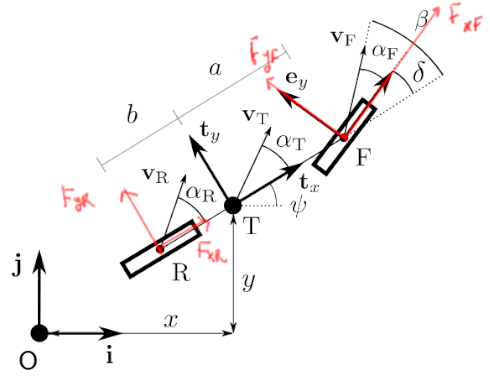
\includegraphics[scale = 0.7]{im_model.png}
    \caption{Bicycle model}
    \label{fig:bmodel}
\end{figure}

\begin{equation}
\begin{aligned}
m_T \ddot{x} = F_{xF} cos(\psi+\delta) + F_{xR} cos(\psi) - F_{yF} sin(\psi+\delta) - F_{yR} sin(\psi) \\
m_T \ddot{y} = F_{xF} sin(\psi+\delta) + F_{xR} sin(\psi) + F_{yF} cos(\psi+\delta) + F_{yR} cos(\psi) \\
I_T \ddot{\psi} = F_{xF} a sin(\delta) + F_{yF} a cos(\delta) - F_{yR} b\\\\
\end{aligned}
\end{equation}

\begin{equation}
\begin{aligned}
\alpha_F = arctan(\frac{\dot{y}+a\dot{\psi}cos(\psi)}{\dot{x}-a\dot{\psi}sin(\psi)}) - (\delta + \psi)\\
\alpha_R = arctan(\frac{\dot{y}-b\dot{\psi}cos(\psi)}{\dot{x}+b\dot{\psi}sin(\psi)}) - \psi\\\\
\end{aligned}
\end{equation}

At first, as state vector this has been used:

\begin{equation}
\begin{aligned}
z1 = x\\
z2 = y\\
z3 = \psi\\
z4 = \dot{x}\\
z5 = \dot{y}\\
z6 = \dot{\psi}\\\\
\end{aligned}
\end{equation}

So that

\begin{equation}
\begin{aligned}
\dot{z_1} = z_4 \\
\dot{z_2} = z_5 \\
\dot{z_3} = z_6 \\
\dot{z_4} = \frac{F_{xF} cos(z_3+\delta) + F_{xR} cos(z_3) - F_{yF} sin(z_3+\delta) - F_{yR} sin(z_3)}{m_T} \\
\dot{z_5} = \frac{F_{xF} sin(z_3+\delta) + F_{xR} sin(z_3) + F_{yF} cos(z_3+\delta) + F_{yR} cos(z_3)}{m_T} \\
\dot{z_6} = \frac{F_{xF} a sin(\delta) + F_{yF} a cos(\delta) - F_{yR} b}{I_T} \\\\
\end{aligned}
\end{equation}

With slip angles

\begin{equation}
\begin{aligned}
\alpha_F = arctan(\frac{z_5+a z_6 cos(z_3)}{z_4-a z_6 sin(z_3)}) - (\delta + z_3)\\
\alpha_R = arctan(\frac{z_5-b z_6 cos(z_3)}{z_4+b z_6 sin(z_3)}) - z_3\\\\
\end{aligned}
\end{equation}

Now instead of using $\dot{x}$ and $\dot{y}$, $v_T$ and $\beta$ have been used. The trasformations are the following: 

\begin{equation}
\begin{aligned}
\dot{x} = v_T cos(\psi + \beta)\\
\dot{y} = v_T sin(\psi + \beta)\\\\
\ddot{x} = \dot{v_T} cos(\psi + \beta) - v_T (\dot{\psi} + \dot{\beta}) sin(\psi + \beta)\\
\ddot{y} = \dot{v_T} sin(\psi + \beta) + v_T (\dot{\psi} + \dot{\beta}) cos(\psi + \beta)\\\\
\end{aligned}
\end{equation}

Substituting and simplyfing with the help of Matlab

\begin{equation}
\begin{aligned}
\dot{v_T} = \frac{F_{xF} cos(\beta-\delta) + F_{xR} cos(\beta) + F_{yF} sin(\beta-\delta) + F_{yR} sin(\beta)}{m_T} \\
\dot{\beta} = \frac{-F_{xF} sin(\beta-\delta) - F_{xR} sin(\beta) + F_{yF} cos(\beta-\delta) + F_{yR} cos(\beta) - m_T v_T \dot{\psi}}{m_T v_T} \\
\ddot{\psi} = \frac{F_{xF} a sin(\delta) + F_{yF} a cos(\delta) - F_{yR} b}{I_T} \\\\
\end{aligned}
\end{equation}

\begin{equation}
\begin{aligned}
\alpha_F = arctan(\frac{v_T sin(\beta) + a\dot{\psi}}{v_T cos(\beta)}) - \delta\\
\alpha_R = arctan(\frac{v_T sin(\beta) - b\dot{\psi}}{v_T cos(\beta)}) \\\\
\end{aligned}
\end{equation}

The new state and the state equations are

\begin{equation}
\begin{aligned}
x1 = x\\
x2 = y\\
x3 = \psi\\
x4 = v_T\\
x5 = \beta\\
x6 = \dot{\psi}\\\\
\dot{x_1} = x_4 cos(x_3 + x_5)\\
\dot{x_2} = x_5 sin(x_3 + x_5)\\
\dot{x_3} = x_6 \\
\dot{x_4} = \frac{F_{xF} cos(x_5-\delta) + F_{xR} cos(x_5) + F_{yF} sin(x_5-\delta) + F_{yR} sin(x_5)}{m_T} \\
\dot{x_5} = \frac{-F_{xF} sin(x_5-\delta) - F_{xR} sin(x_5) + F_{yF} cos(x_5-\delta) + F_{yR} cos(x_5) - m_T x_4 x_6}{m_T x_4} \\
\dot{x_6} = \frac{F_{xF} a sin(\delta) + F_{yF} a cos(\delta) - F_{yR} b}{I_T} \\\\
\end{aligned}
\end{equation}

\section{Pacejka tyre model}

The following Pacejka tyre model (Magic Formula '94) has been used, taking as inputs the tyre slip angle $\alpha$ ($\alpha_F$ and $\alpha_R$) and the vertical load $F_z$ on the tyre (respectively $l_F*F_z$ and $l_R*F_z$, where $l_F$ and $l_R$ are coefficients to distribute the load between front wheel and rear wheel, such that $l_F+l_R=1, l_F>=0, l_R>=0$).

\begin{equation}
\begin{aligned}
F_y = D sin (C arctan (B_{x1} - E (B_{x1} - arctan(B_{x1})))) + V\\\\
\end{aligned}
\end{equation}

With

\begin{equation}
\begin{aligned}
C = a_0\\
D = F_z (a_1 F_z + a_2) (1 - a_{15} \gamma^2)\\
BCD = a_3 sin (2 arctan(\frac{F_z}{a_4})) (1 - a_5 |\gamma|)\\
B = BCD / CD\\
E = (a_6 F_z + a_7) (1 - (a_{16} \gamma + a_{17})sign(\alpha+H))\\
H = a_8 F_z + a_9 + a_{10} \gamma\\
V = a_{11}F_z + a_{12} + (a_{13} F_z + a_{14}) \gamma F_z\\
B_{x1} = B (\alpha + H)\\\\
\end{aligned}
\end{equation}

Where $a_i$, i $\in$ \{0,..,17\}, are the parameters of the Pacejka model, whose value and meaning can be seen in the Appendix.

\section{Aerodynamic force}

The \color{red} following \color{black} changes have been done in the previous model to take into account for the aerodynamic force $F_A = \frac{1}{2} \rho C_x S v^2$ in the same direction of $v_T$ but in the opposite side, and $F_{Lift} = \frac{1}{2} \rho C_z S v^2$ that "pushes" the vehicle to be sticked on the ground. In here $S$ is the area of the vehicle on which the air goes through, $C_x, C_z$ are drag coefficients, $\rho$ is the density of the air and $v$ is the velocity of the vehicle

\begin{equation}
\begin{aligned}
..\\
\dot{x_4} = \frac{F_{xF} cos(x_5-\delta) + F_{xR} cos(x_5) + F_{yF} sin(x_5-\delta) + F_{yR} sin(x_5) \color{red} -\frac{1}{2} \rho C_x S x_{4}^2 \color{black}}{m_T} \\
..\\
\end{aligned}
\end{equation}
\begin{equation}
\begin{aligned}
F_z = mg \color{red} + \frac{1}{2} \rho C_z S x_{4}^2 \color{black} \\\\
\end{aligned}
\end{equation}

\section{Fuel consumption}

The \color{red} following \color{black} changes have been done in the previous model to take fuel consumption into account. A simplified version has been used, in which the Power is computed ($P_e$) and multiplied by a coefficient ($C_{fuel}$) that expresses the relation among mass loss (in terms of fuel consumption) and power provided

\begin{equation}
\begin{aligned}
\color{red} P_e = (F_{xF} + F_{xR}) x_4 \color{black}, F_{xF}>=0, F_{xR}>=0 \\
\color{red} \dot{m} = P_e C_{fuel} \color{black}\\
\end{aligned}
\end{equation}

\section{Tyre wear}

The \color{red} following \color{black} have been added in the previous model to take into account for wear of the rubber compound of the tyre. The model is called Archard model, and it makes use of the vertical pression ($P_z = \frac{F_z}{Area}$), the longitudinal sliding velocity of the wheels ($v_{xF}$ and $v_{xR}$) and some parameters (such as $K_{wear}$ and $H$). The model output is the wear depth over the time ($\dot{h}$), that will be then converted into $mm^3$ of wasted material.\\The model has been converted in order to take into account, instead of the sliding velocity, the forces on the wheels, thus the parameters have been re-modulated too.\\
Here the modified Archard model formulation is shown

\begin{equation}
\begin{aligned}
\color{red} \dot{h_i} = \frac{K_{wear} P_{load} \sqrt{F_{xi}^2+F_{yi}^2}}{H} \color{black}\\
\text{where i $\in$ \{F, R\}}
\end{aligned}
\end{equation}

\section{Banking}

Taking into account the shape of the road we introduce other terms in the model equations. As can be seen in figure \ref{fig:contribmg} and \ref{fig:basedonpos} we are able to find the term whose projection will be summed up in the previous dynamic equations, that is the $mg$ term, that multiplied by $sin(\gamma)$ will be directed as the perpendicular to the vehicle direction.\\\\ 
As can be seen from those figures, the contribution of this lateral force acting on the vehicle will add some new terms in the equations of the model.
Along the direction of $v_T$ the contribution of the force is \color{red} $mgsin(\gamma)sin(\beta)$\color{black}, while on the orthogonal direction it is
represented by the force \color{red} $mgsin(\gamma)cos(\beta)$\color{black}.\\\\
\\
\begin{figure}[h!]
    \centering
    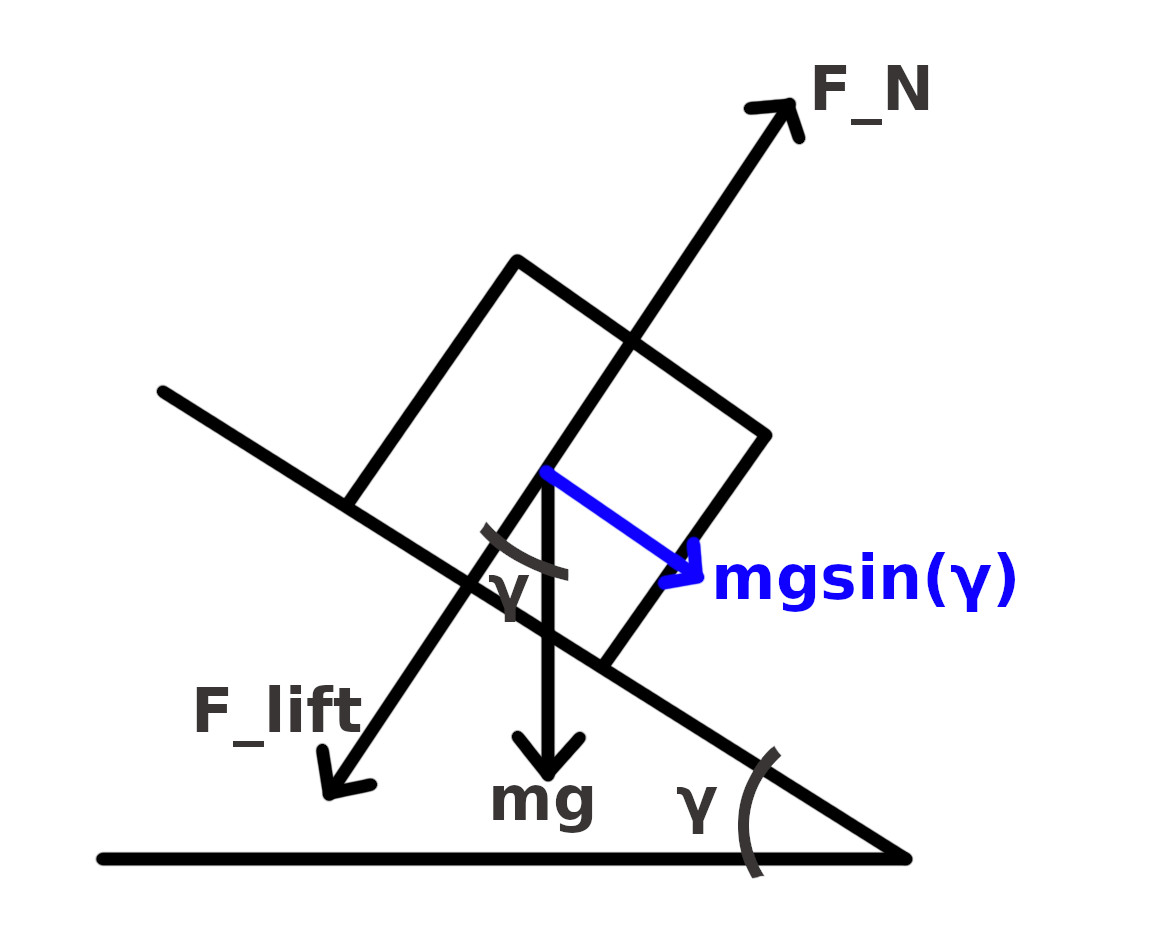
\includegraphics[scale = 0.2]{equilibriumOnZAxis.jpg}
    \caption{Contribution of mg}
    \label{fig:contribmg}
\end{figure}
\begin{figure}[h!]
    \centering
    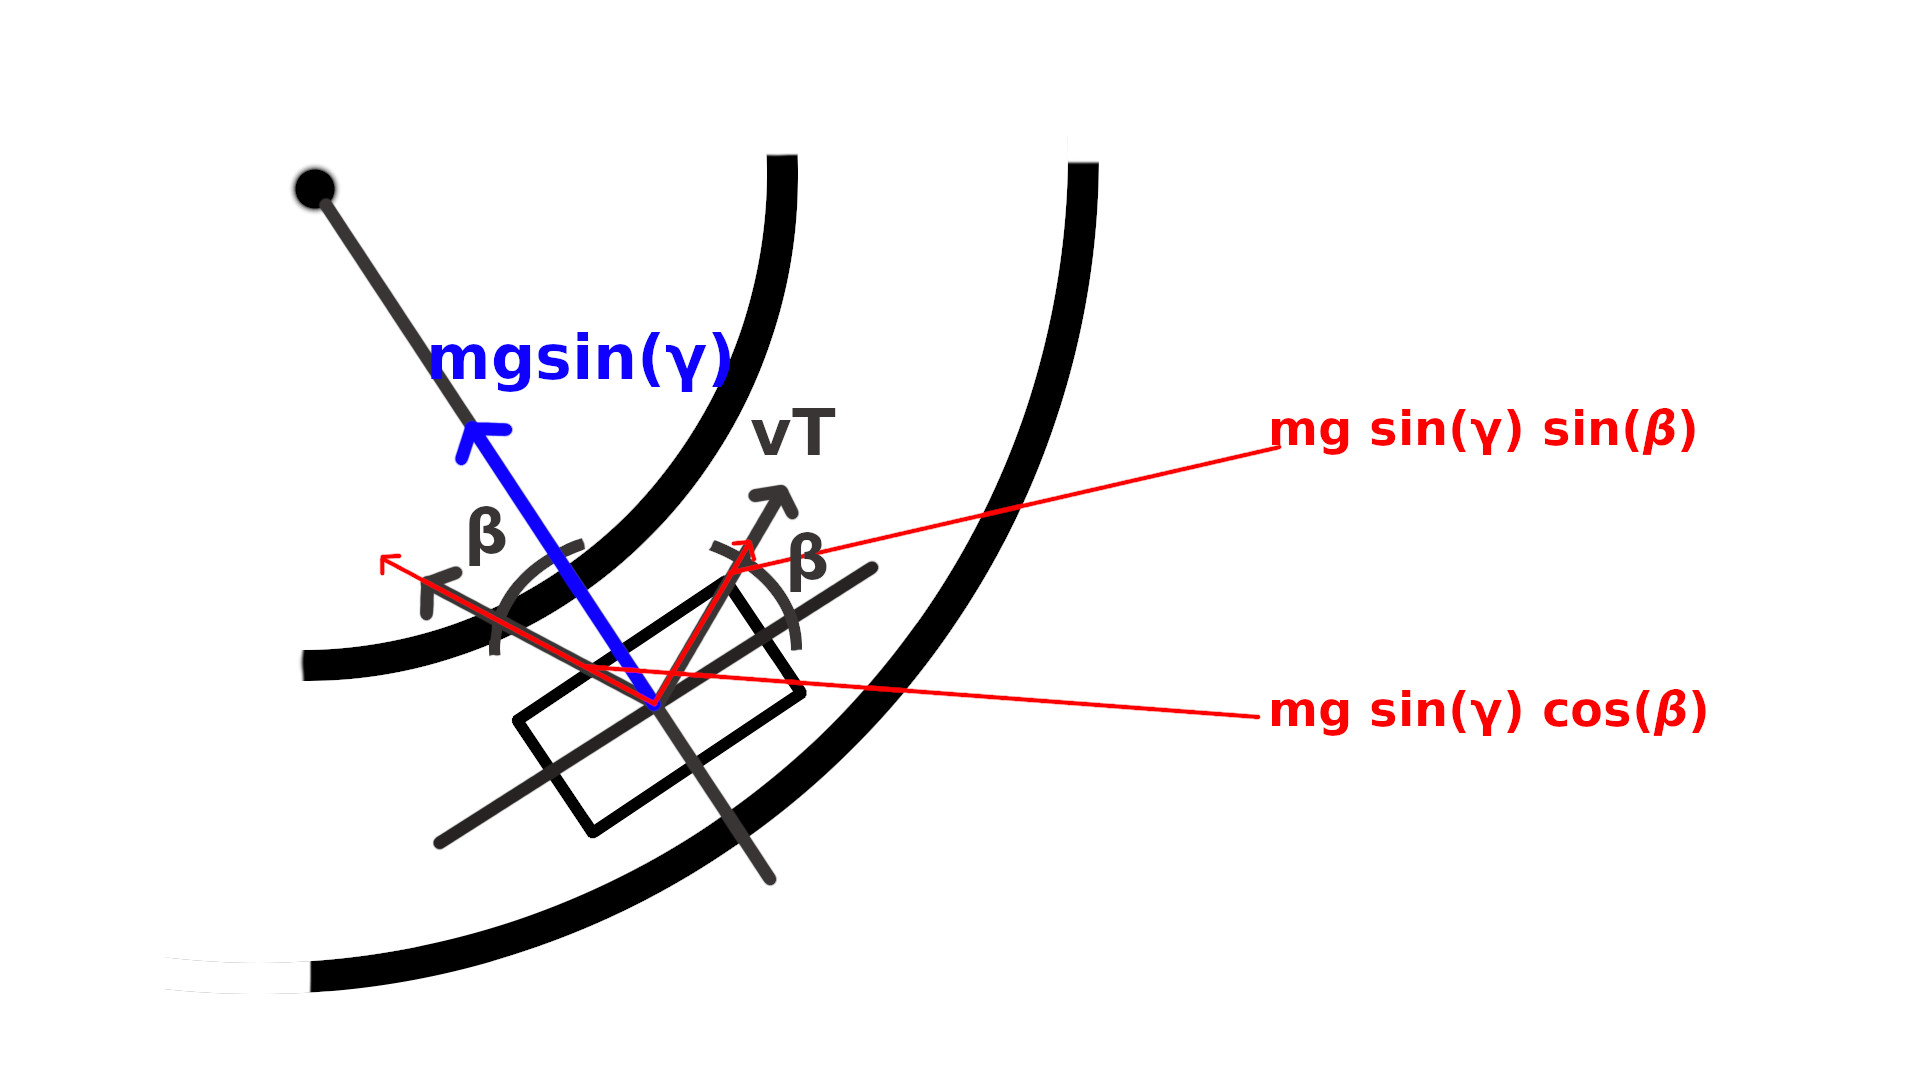
\includegraphics[scale = 0.2]{basedOnPosition.jpg}
    \caption{Terms affecting the model equations}
    \label{fig:basedonpos}
\end{figure}

In the end, the final equations will be:
\begin{equation}
\begin{aligned}
\\
\dot{x_4} = \frac{F_{xF} cos(x_5-\delta) + F_{xR} cos(x_5) + F_{yF} sin(x_5-\delta) + F_{yR} sin(x_5) -\frac{1}{2} \rho C_x S v^2 \color{red} + mgsin(\gamma) sin(x_5) \color{black}}{m_T} \\
\\
\dot{x_5} = \frac{-F_{xF} sin(x_5-\delta) - F_{xR} sin(x_5) + F_{yF} cos(x_5-\delta) + F_{yR} cos(x_5) - m_T x_4 x_6 \color{red} + mgsin(\gamma) cos(x_5) \color{black}}{m_T x_4} \\
\end{aligned}
\end{equation}


\section{Friction ellipse and wear}
Coming to the conclusion of our model, we took in consideration also the physical relation between longitudinal and lateral forces through the friction ellipse

\begin{equation}
\begin{aligned}
{(\frac{F_x}{F_{x,max}})}^2 + {(\frac{F_y}{F_{y,max}})}^2 = 1
\end{aligned}
\end{equation}

In particular, $F_{x,max}$ and $F_{y,max}$ are respectively the maximum longitudinal and lateral forces, that are are calculated through the Pacejka parameters, being $D + V$ the point of max of the tyre model. Here we recall that: 

\begin{equation}
\begin{aligned}
D_{lat} = F_z (a_1 F_z + a_2) (1 - a_{15} \gamma^2)\\
V_{lat} = a_{11}F_z + a_{12} + (a_{13} F_z + a_{14}) \gamma F_z\\\\
D_{long} = F_z (b_1 F_z + b_2)\\
V_{long} = b_{11}F_z + b_{12} \\\\
\end{aligned}
\end{equation}

Thus as we can see, the maximum longitudinal and lateral forces are functions of the vertical load $F_z$.\\(Note: different parameters are used for longitudinal and lateral Pacejka, in particular $a_i$ is referred to the lateral one while $b_i$ to the longitudinal one).\\\\
In this way the ellipse is defined, but, taking in consideration the wear $h$ the ellipse is scaled. Thus, at the end, $F_{x,max}$ and $F_{y,max}$ are functions of $F_z$ and $h$, specifically:

\begin{equation}
\begin{aligned}
F_{x,max} = (D_{long} + V_{long}) \frac{1}{w_1 h + w_2}\\
F_{y,max} = (D_{lat} + V_{lat}) \frac{1}{w_1 h + w_2}
\end{aligned}
\end{equation}

Where $w_1$ and $w_2$ are parameters opportunely chosen. In this way the more the wear, the more the ellipse is shrunk.\\\\
The ellipse is saying us which is the maximum lateral force wrt the given $F_x$ in input. Thus, finally, the output of the lateral Pacejka is scaled, so to have the peak value ($D_{lat}+V_{lat}$) equal to the value given by the ellipse. To do so, the D value of the Pacejka is directly fed as input to the model through the output of the ellipse.\\Following image tries to clarify the steps detailed so far.

\begin{figure}[h!]
    \centering
    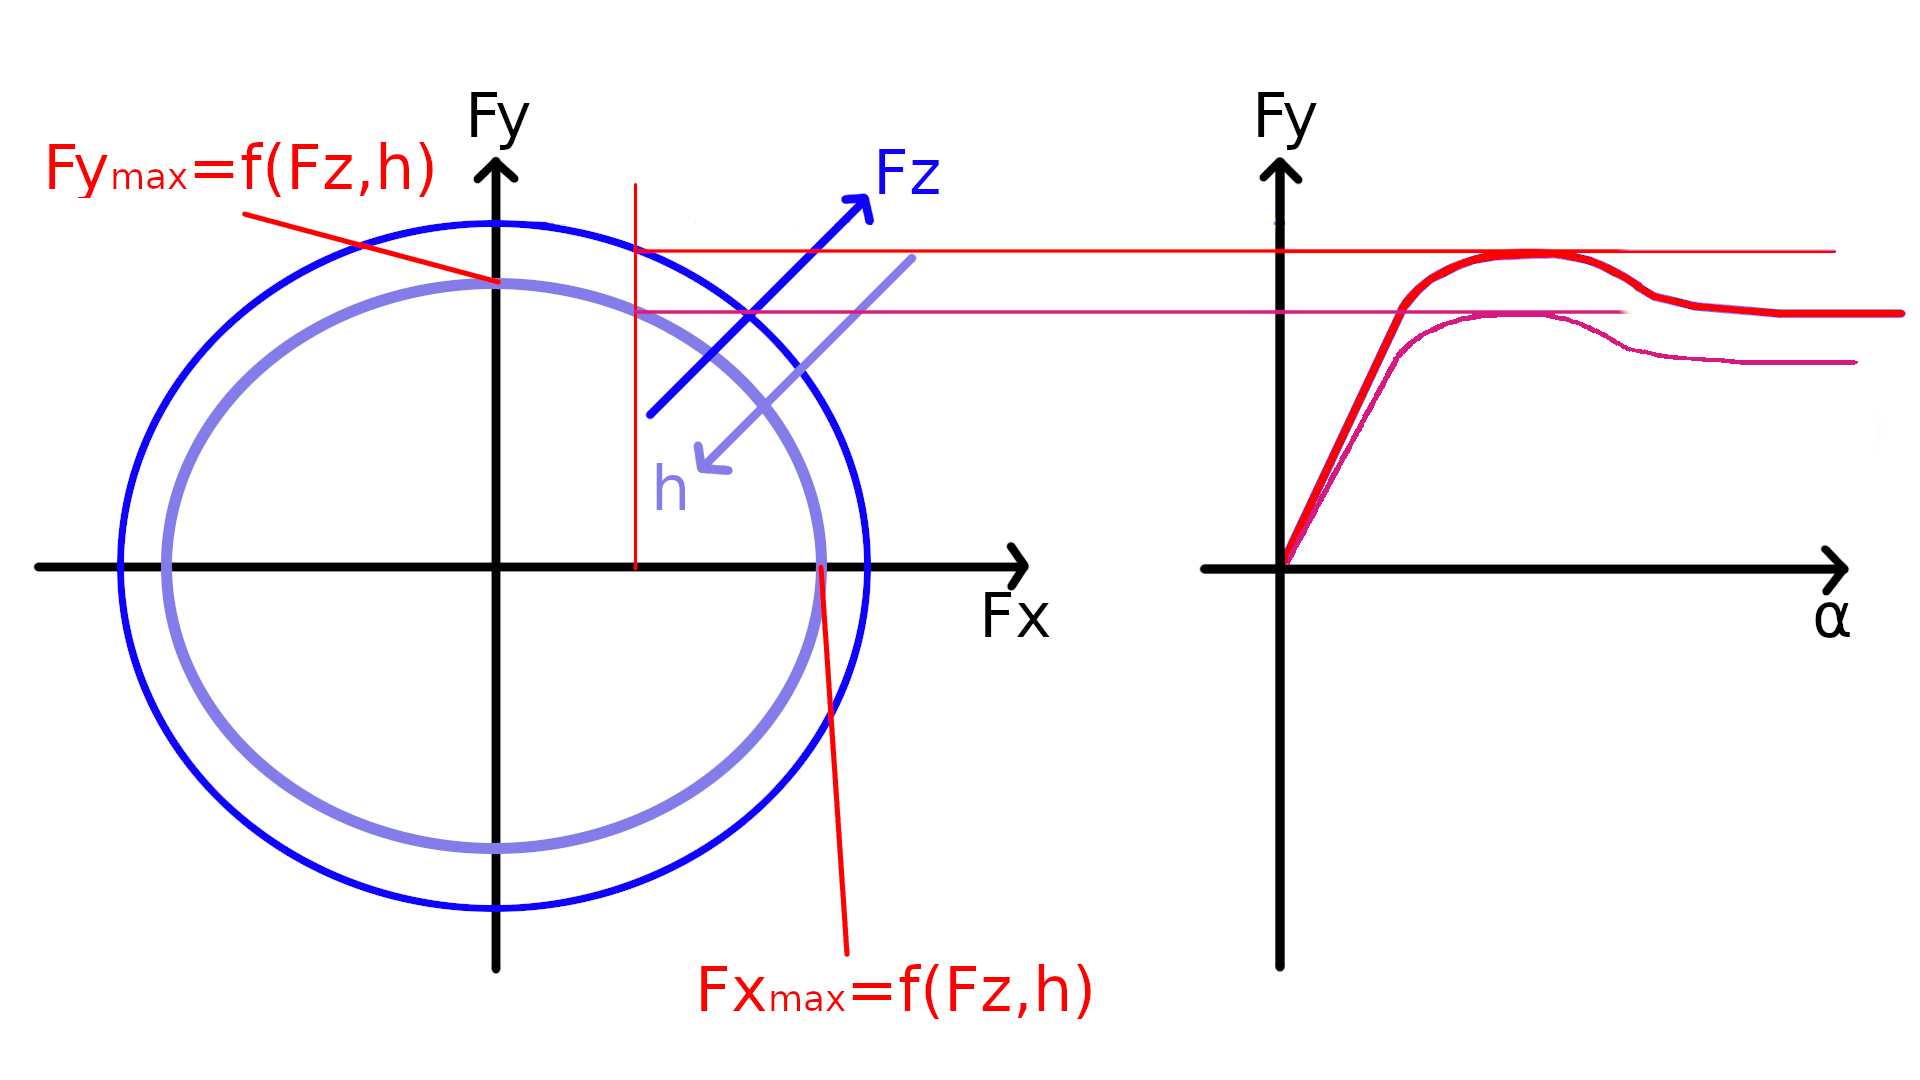
\includegraphics[scale = 0.17]{ellisse.png}
    \caption{Friction ellipse and wear effects}
    \label{fig:ellisse}
\end{figure}

\newpage

\section{Slipstream}
In our model we also considered the slipstream effect. Some thresholds have been defined to establish if the vehicle is undergoing the slipstream condition. These thresholds take into account both front and rear distance of two different vehicles and also their alignment degree: below these values, the slipstream is considered to be effective. This leads to have a lower air density coefficient $\rho$ in the aerodynamic force formula, that physically represents a lower opponent aerodynamic force. All the used coefficients can be found in the appendix. 

\section{Simulations}
Different simulations have been run to validate qualitatively the presented model and to highlight its most relevant features. Among the others, 5 simulations are considered to be the most representative and are shown in the following. For each simulation only the most relevant graphs have been shown. For a complete overview of the simulations we refer to this link \url{https://github.com/cvalore/simulations\_logs} where it is possible to find the logs and all graphs related to these simulations.
Note: In all the simulations the input $\delta$ is reported, that is the wheel-angle although we directly fed the steer-angle. They can be reciprocally easy calculated knowing that the steering ratio $\frac{steer\_angle}{wheel\_angle} = 10$.


\subsection{Simulation 1 - Non-accelerating straight path}
In this preliminary simulation the aim was to test the correctness of the various figures of merit in a flying start situation with an initial velocity of $20[m/s]$ and nothing else. Provided inputs are $F_x = 0 [N]$, $\delta = 0 [rad]$, simulation time = $30 [s]$. Banking is not considered. 
\\Although not very significant, this test guarantees that all the internal forces are working correctly. Indeed, the decreasing of the acceleration and velocity due to the aerodynamic force can be seen in the figure \ref{fig:sim1_1}. All the other figures are not useful, since all angles, lateral forces, power and mass decreasing factor are zero; also the trajectory is not reported since it is simply a straight line. \\

\begin{figure}[h!]
    \centering
    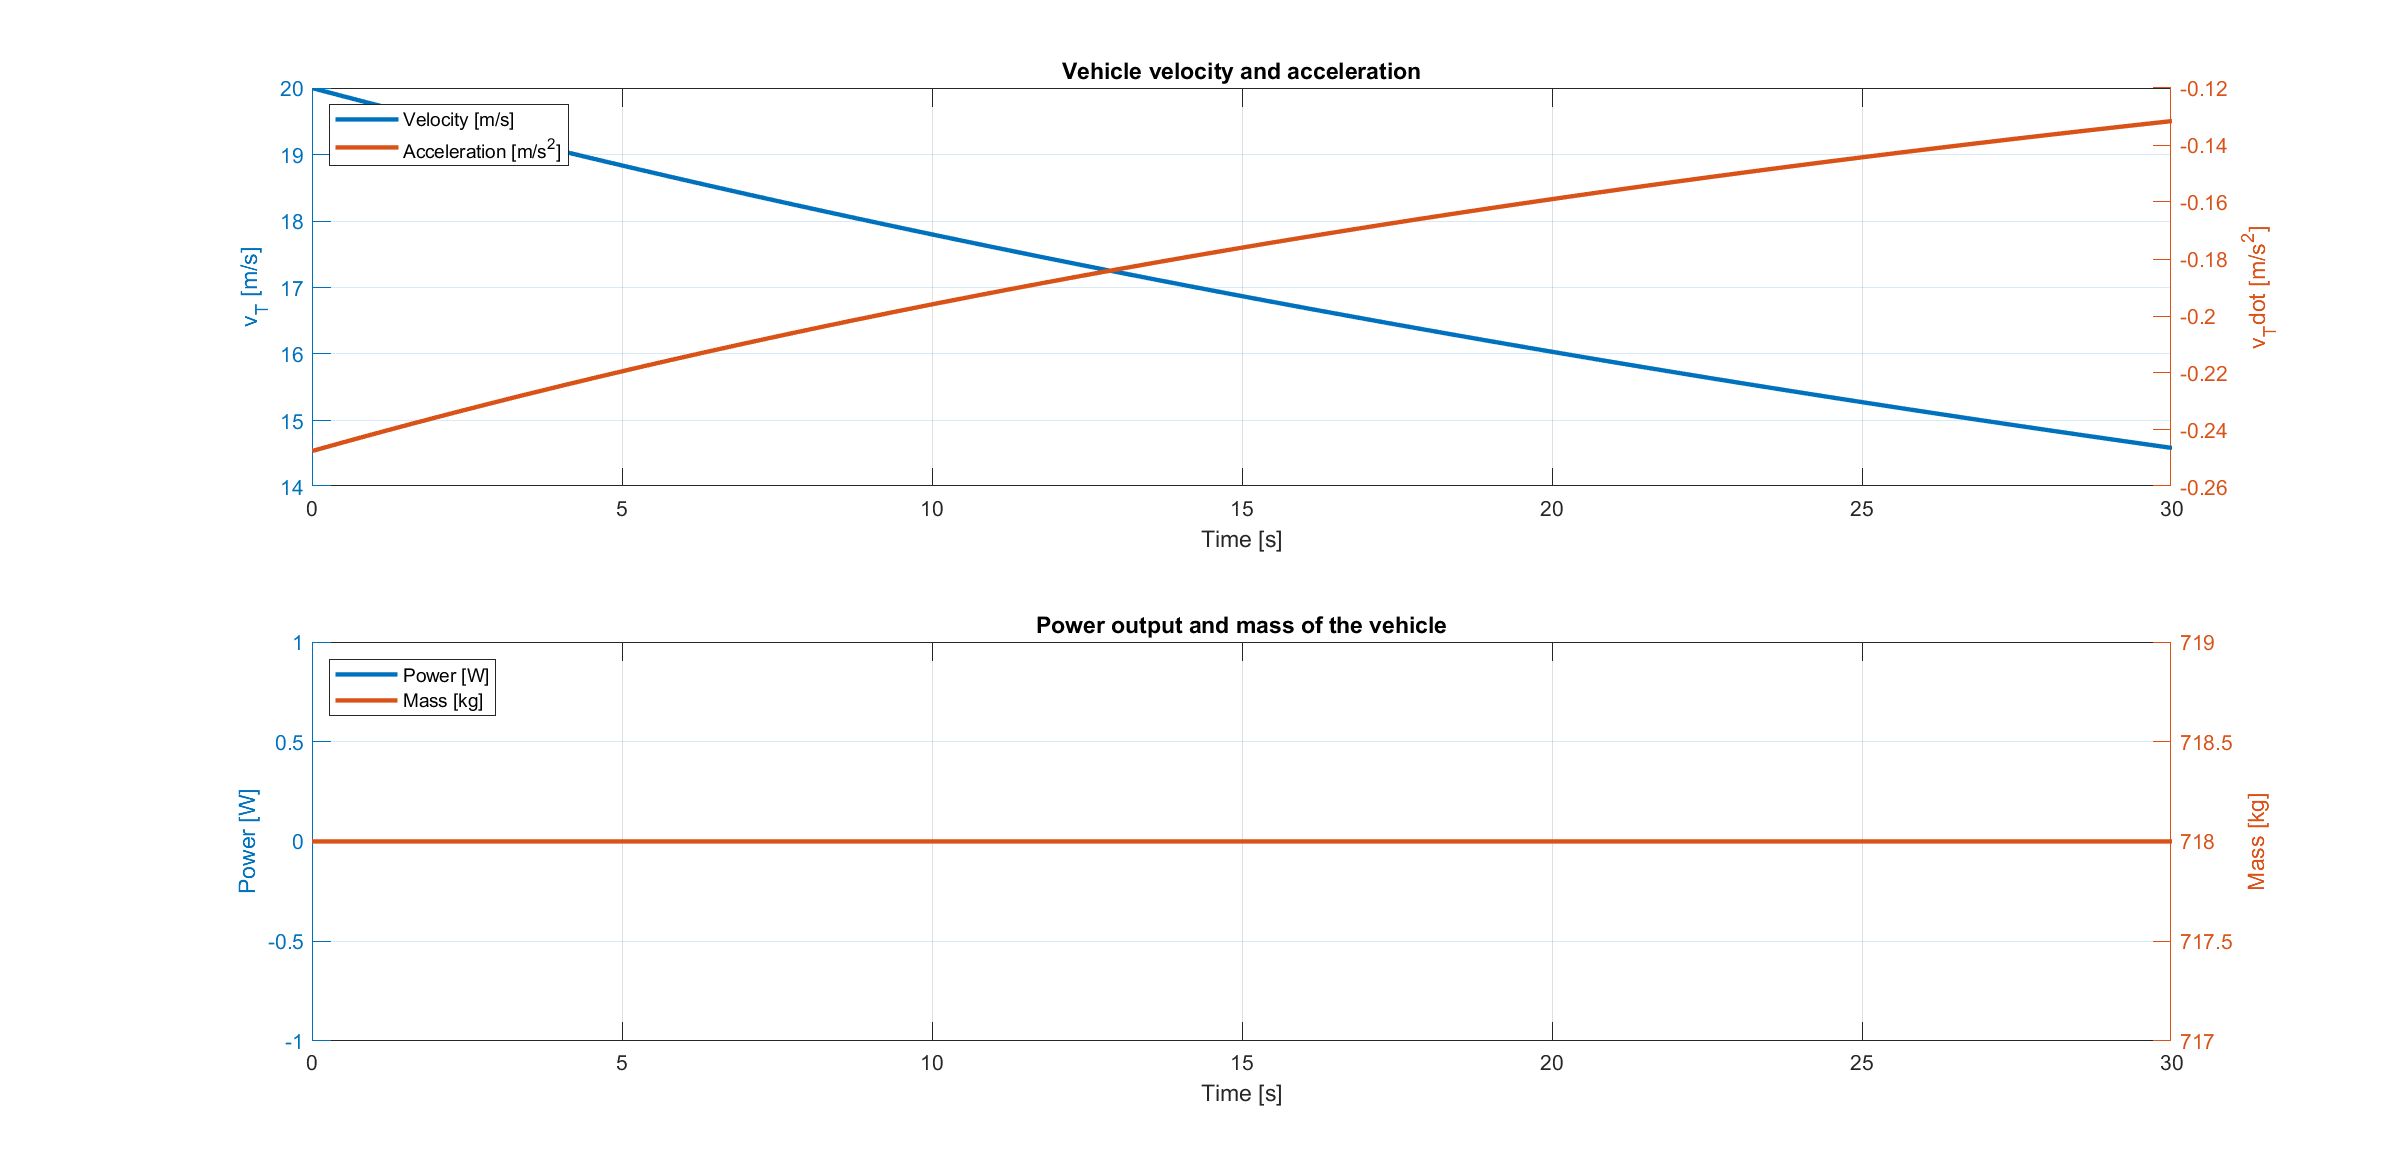
\includegraphics[width=\linewidth]{sim1_vel-power.png}
    \caption{Simulation 1 - velocity, acceleration, power and mass figure}
    \label{fig:sim1_1}
\end{figure}

\subsection{Simulation 2 - Accelerating straight path}
In this preliminary simulation the aim was to test the correctness of the various figures of merit in a situation in which the initial velocity of the vehicle is $0[m/s]$ and there is a constant acceleration. Provided inputs are $F_x = 1000 [N]$, $\delta = 0 [rad]$, simulation time = $30 [s]$. Banking is not considered.
\\Also in this case not every simulation result is shown, since angles and trajectory are, as before, respectively zero and a straight line. The velocity and acceleration figure is shown and it is consistent with the given simulation data; the first one is increasing since there is a constant force applied over all the time interval that makes the acceleration always positive, the second one is decreasing since the applied force is not changing over the time and the aerodynamic force is increasing with the square of the velocity. The figures reported, figures \ref{fig:sim2_1} and \ref{fig:sim2_2} are showing as the tyres wear is increasing with time and how the power is effecting the mass of the vehicle (actually the mass of the fuel) that is decreasing.\\ 
\begin{figure}[h!]
    \centering
    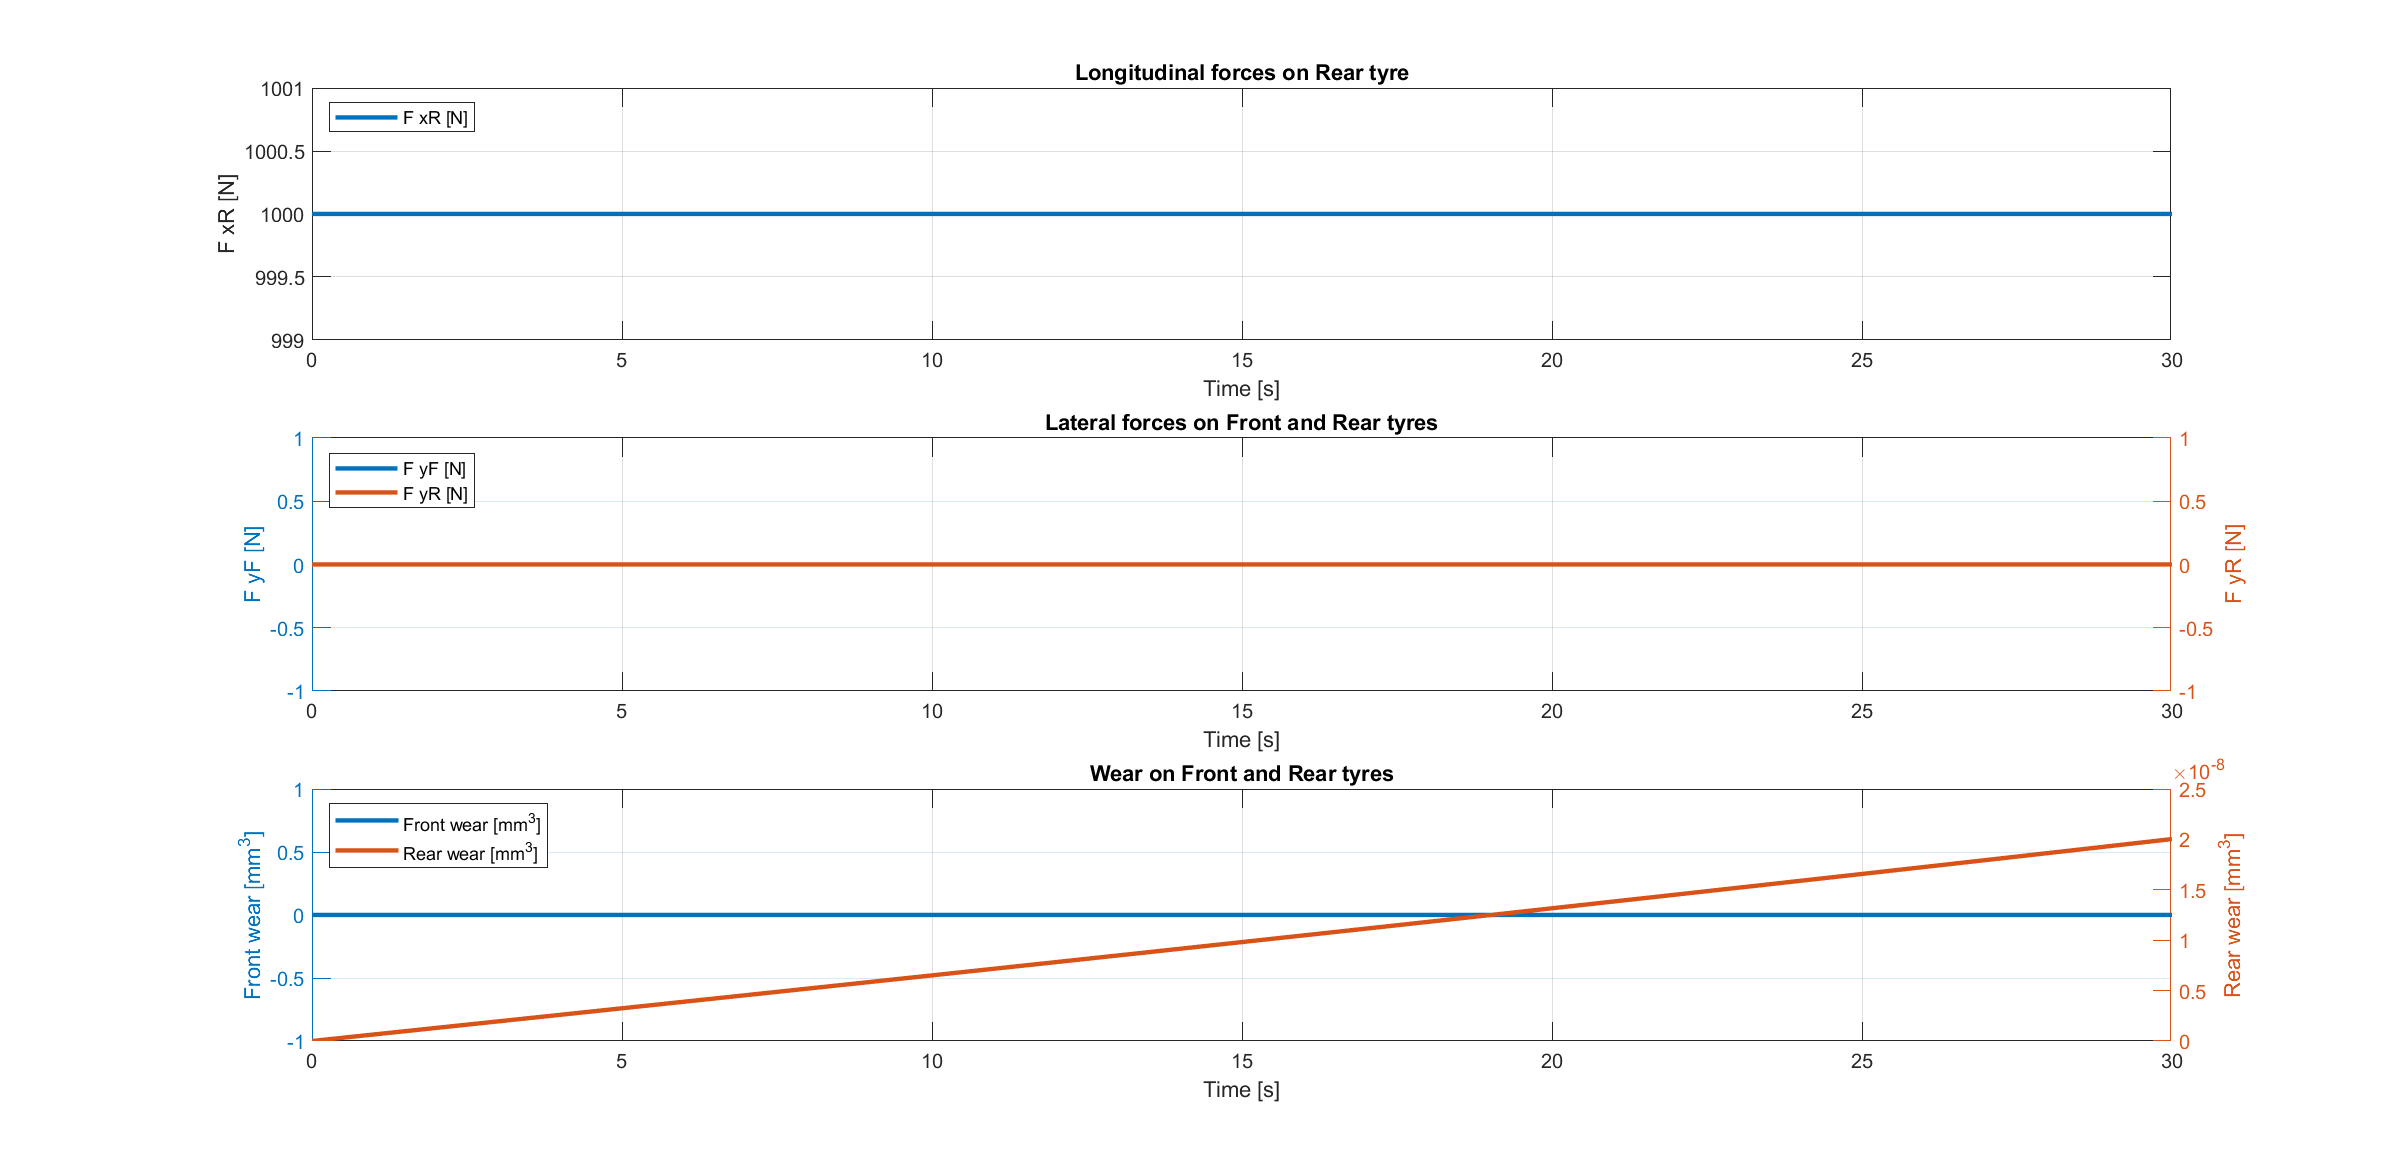
\includegraphics[width=\linewidth]{sim2_force-wear.png}
    \caption{Simulation 2 - forces and tyres wear figure}
    \label{fig:sim2_1}
\end{figure}
\begin{figure}[h!]
    \centering
    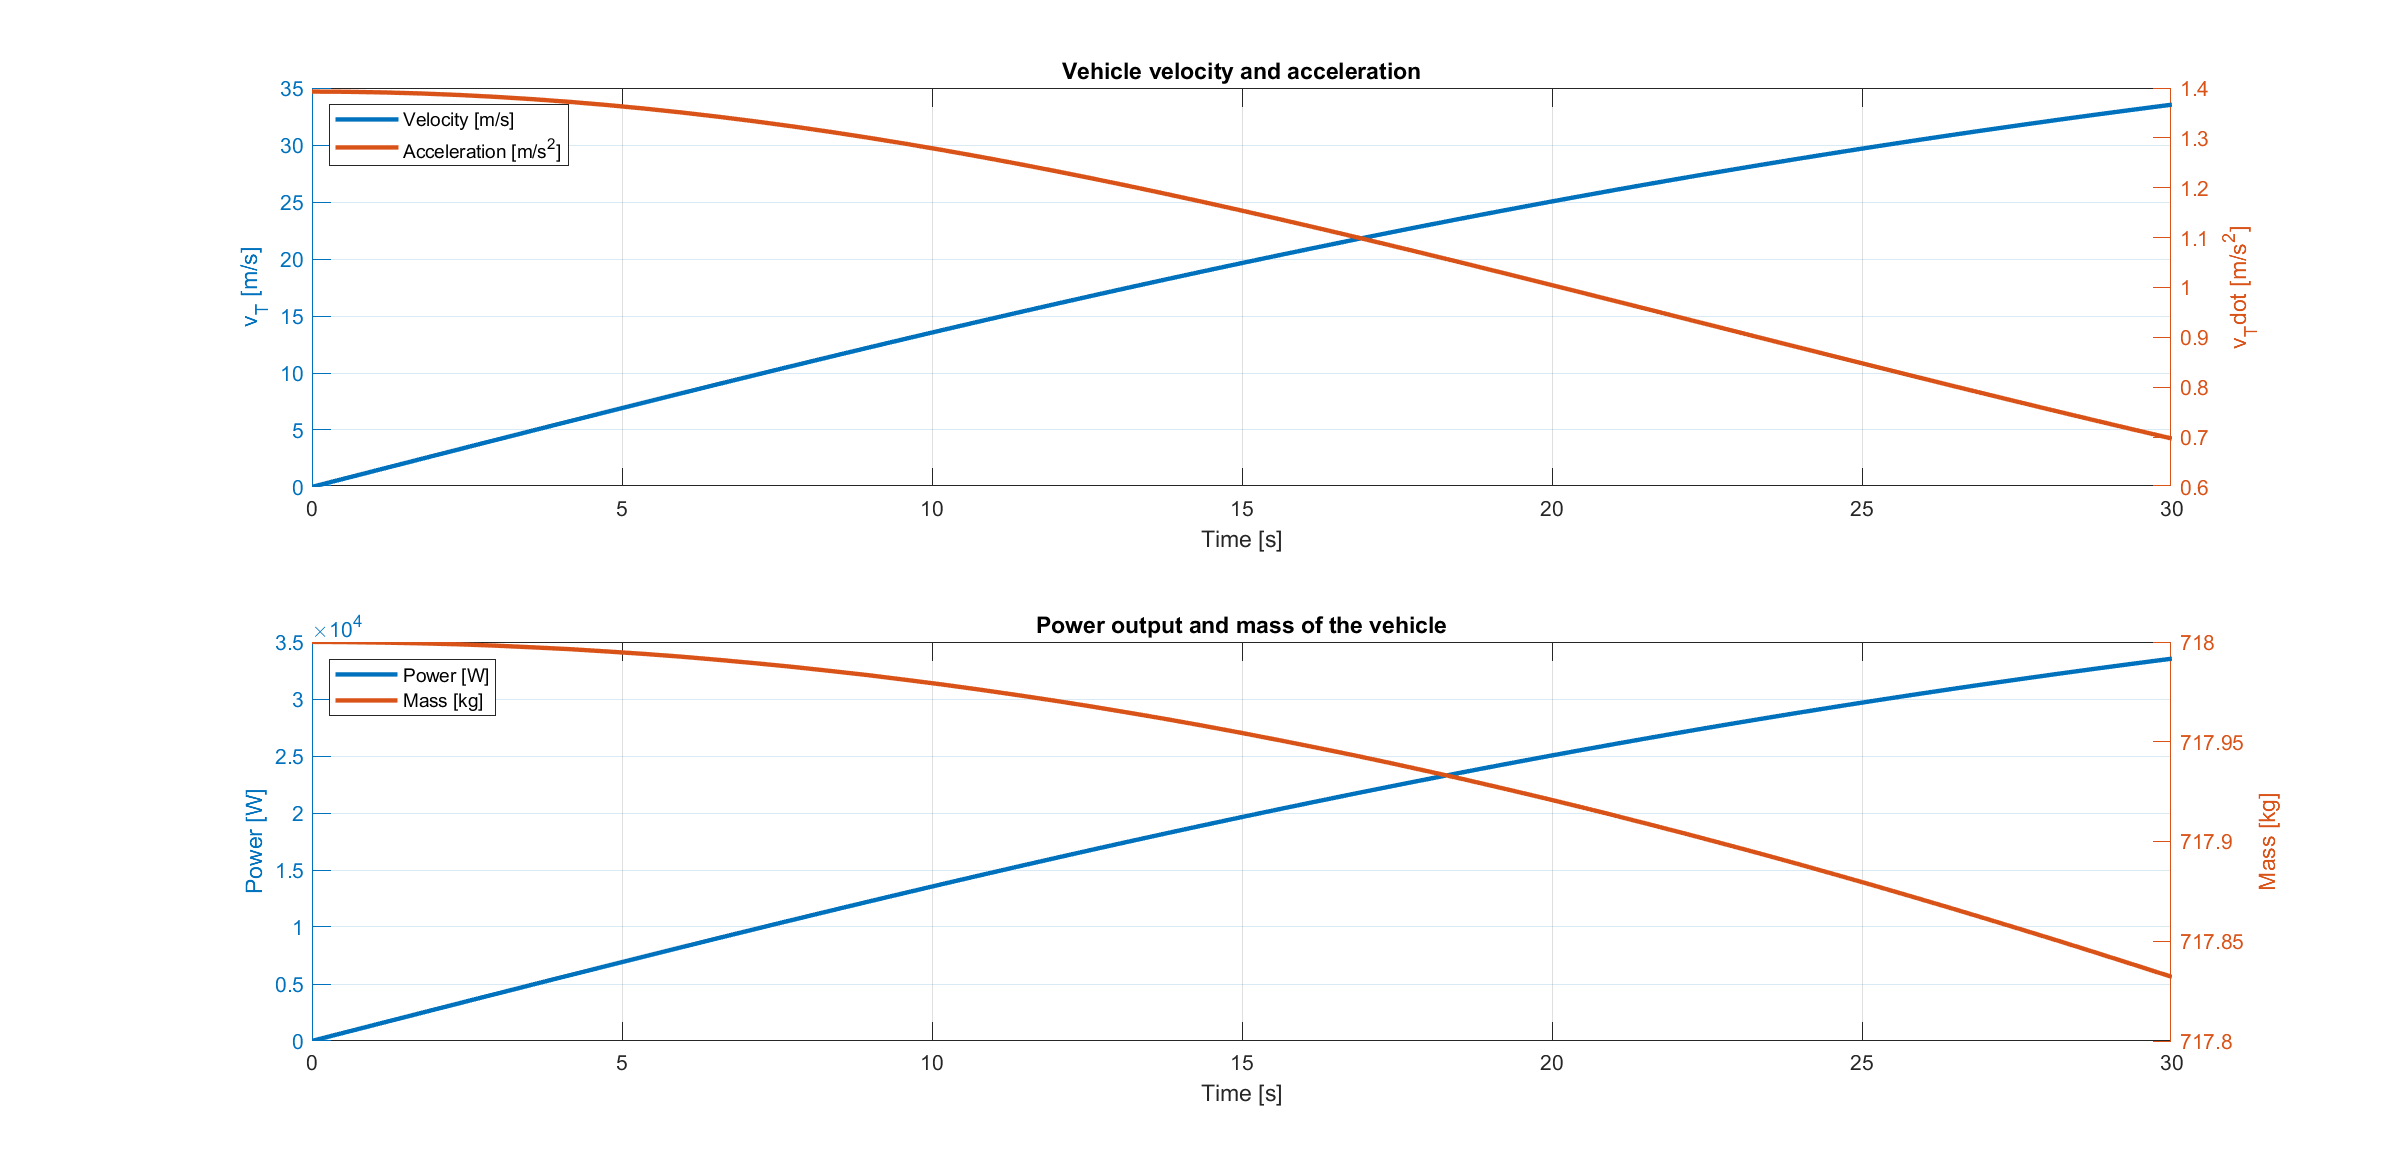
\includegraphics[width=\linewidth]{sim2_vel-power.png}
    \caption{Simulation 2 - velocity, acceleration, power and mass figure}
    \label{fig:sim2_2}
\end{figure}

\subsection{Simulation 3 - Accelerating straight path on a banked road}
In this simulation the aim was to test the correctness of the various figures of merit when the ego vehicle traverses a banked road. Provided inputs are: $F_x = 500 [N]$, $\delta = 0 [rad]$, simulation time = $50 [s]$. 

\begin{figure}[h!]
    \centering
    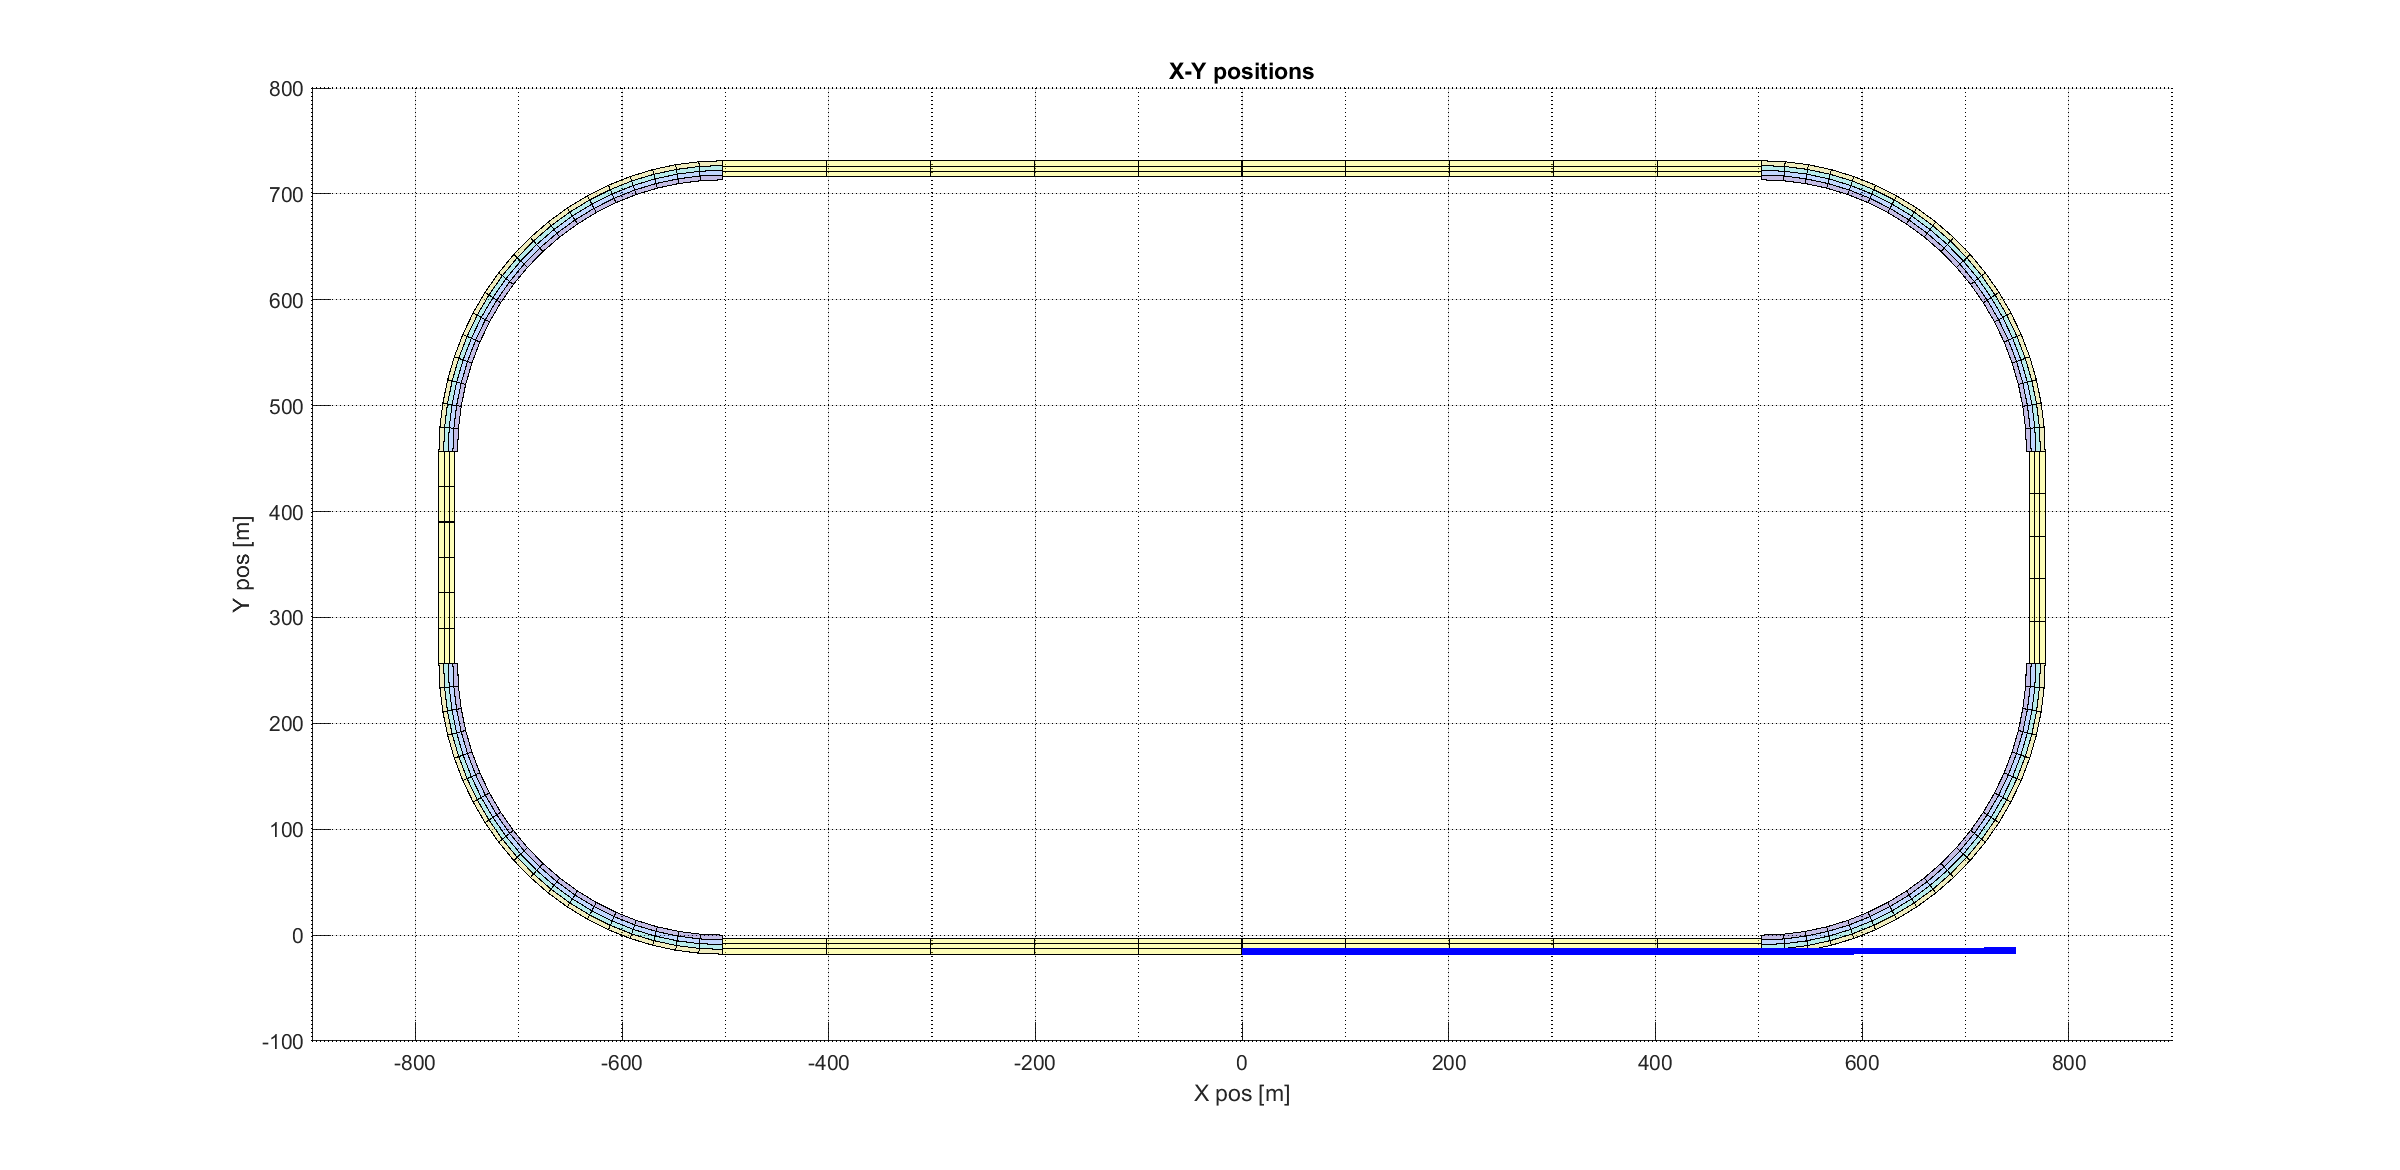
\includegraphics[width=\linewidth]{sim3_trajectory.png}
    \caption{Simulation 3 - trajectory of the vehicle on the banked road}
    \label{fig:sim3_1}
\end{figure}

\begin{figure}[h!]
    \centering
    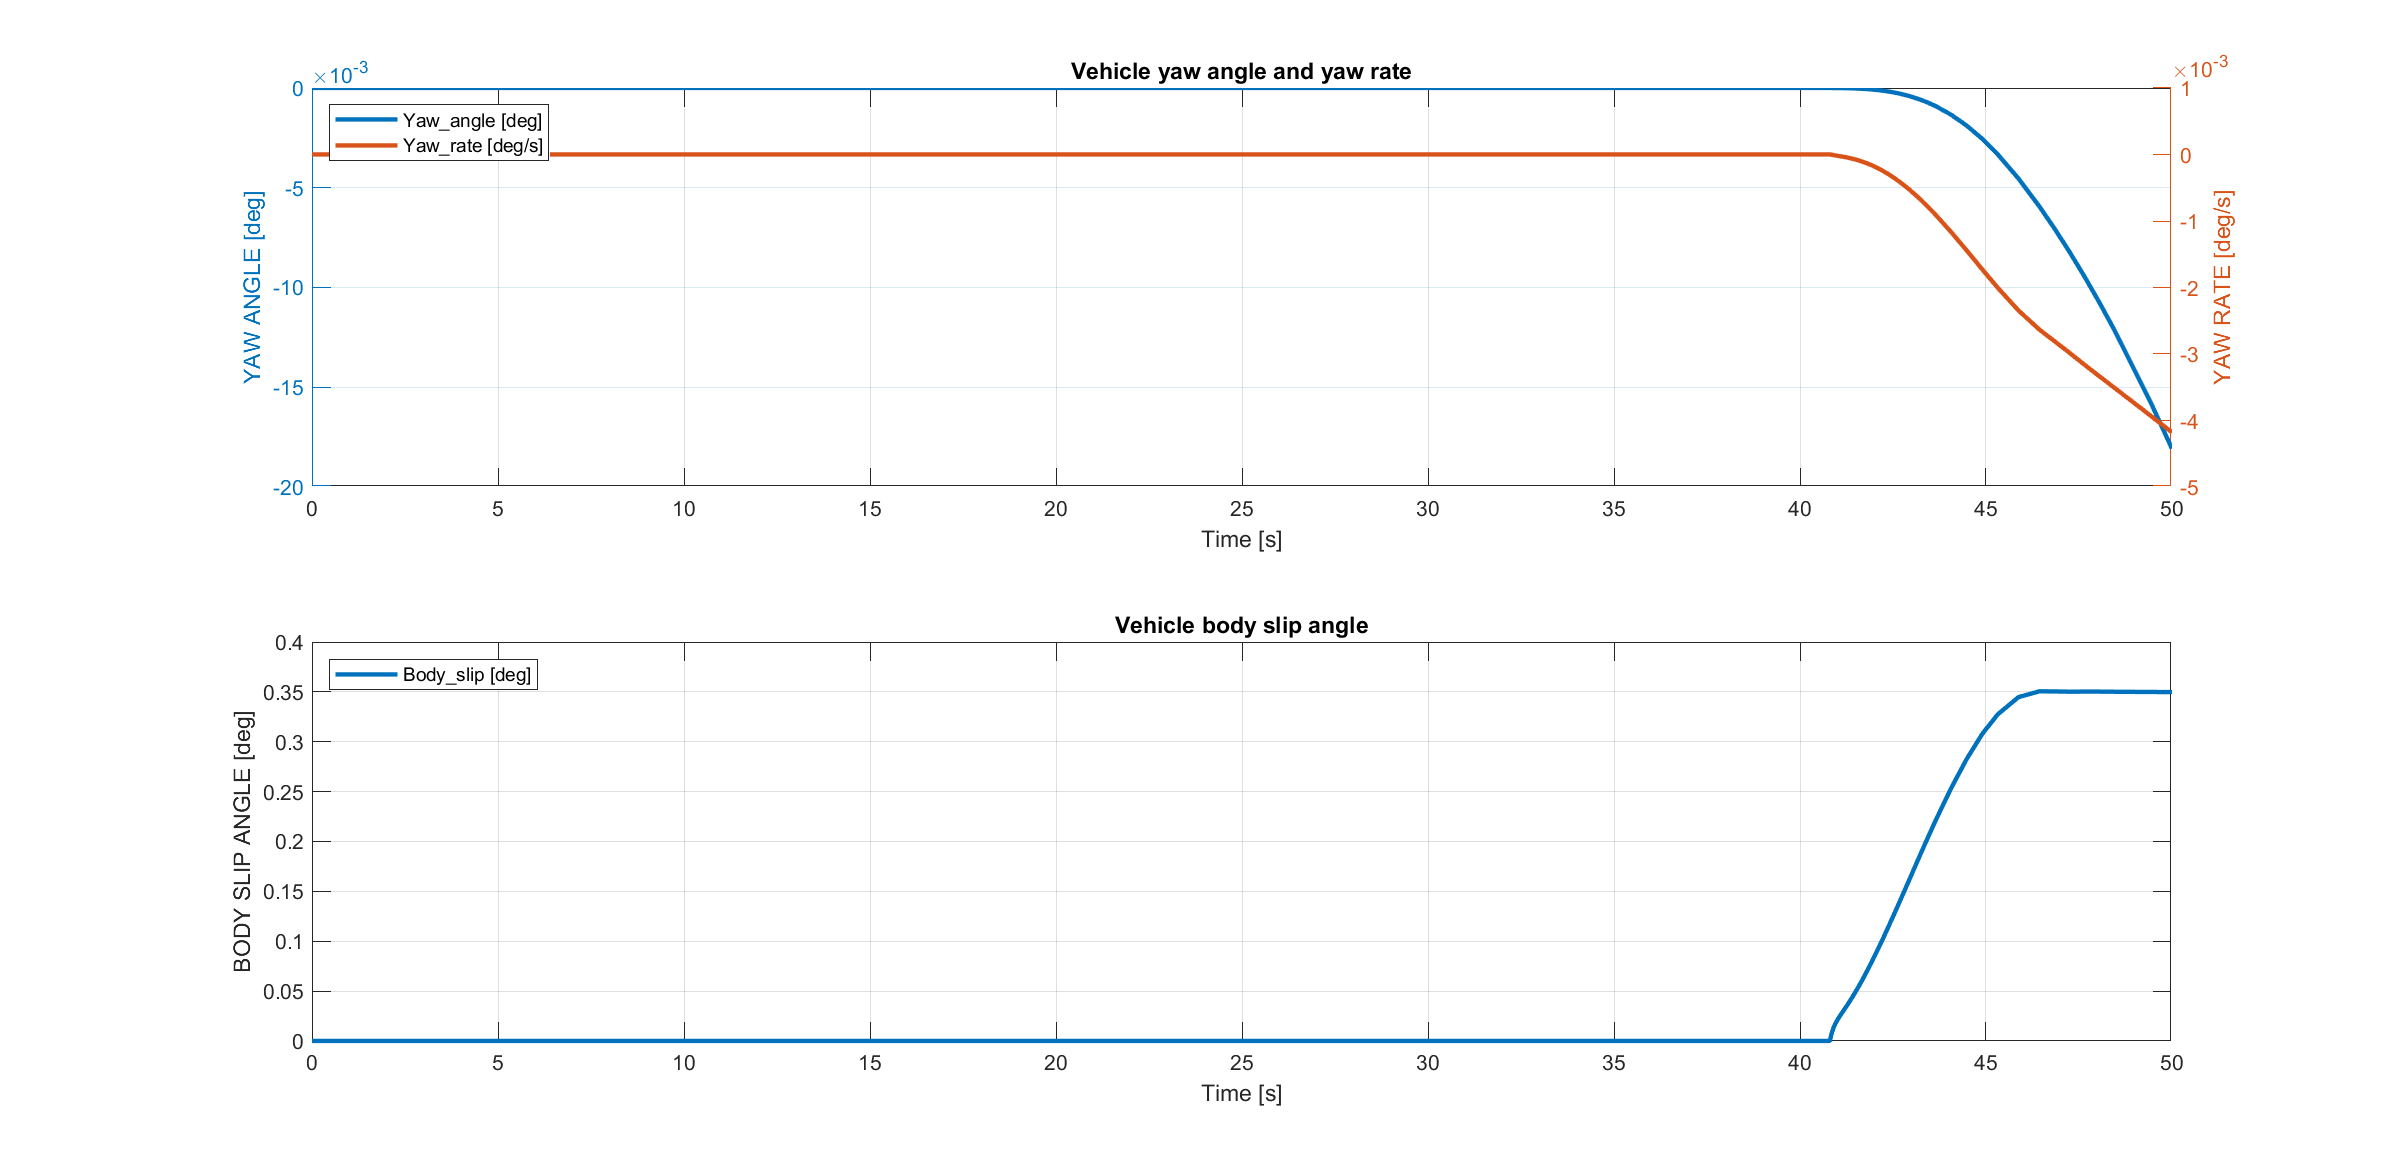
\includegraphics[width=\linewidth]{sim3_angles.png}
    \caption{Simulation 3 - angles figure}
    \label{fig:sim3_2}
\end{figure}

\begin{figure}[h!]
    \centering
    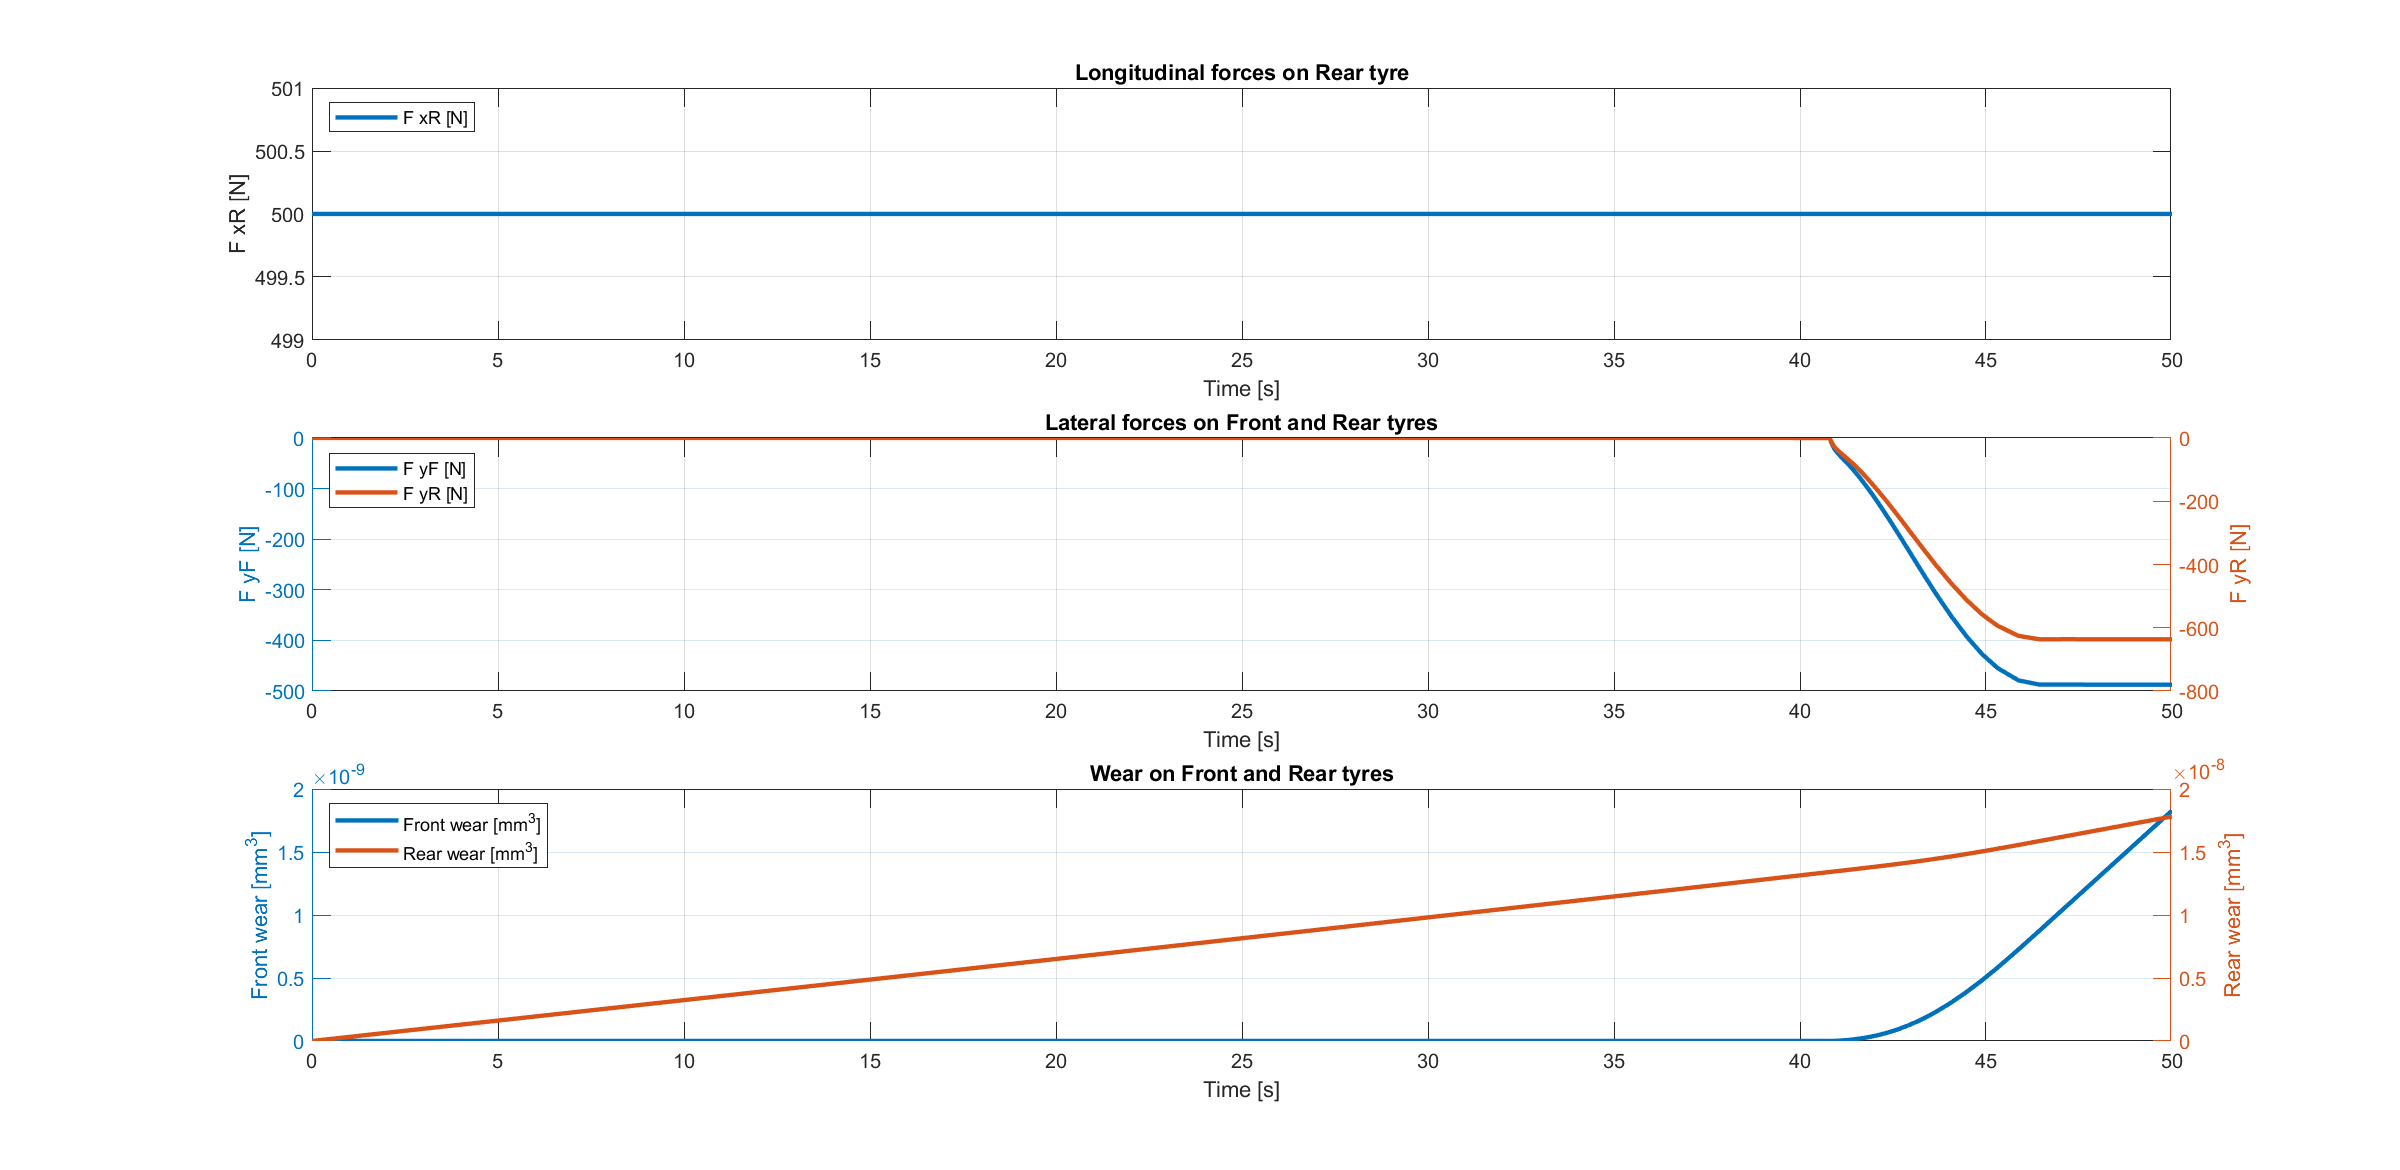
\includegraphics[width=\linewidth]{sim3_force-wear.png}
    \caption{Simulation 3 - forces and tyres wear figure}
    \label{fig:sim3_3}
\end{figure}

\begin{figure}[h!]
    \centering
    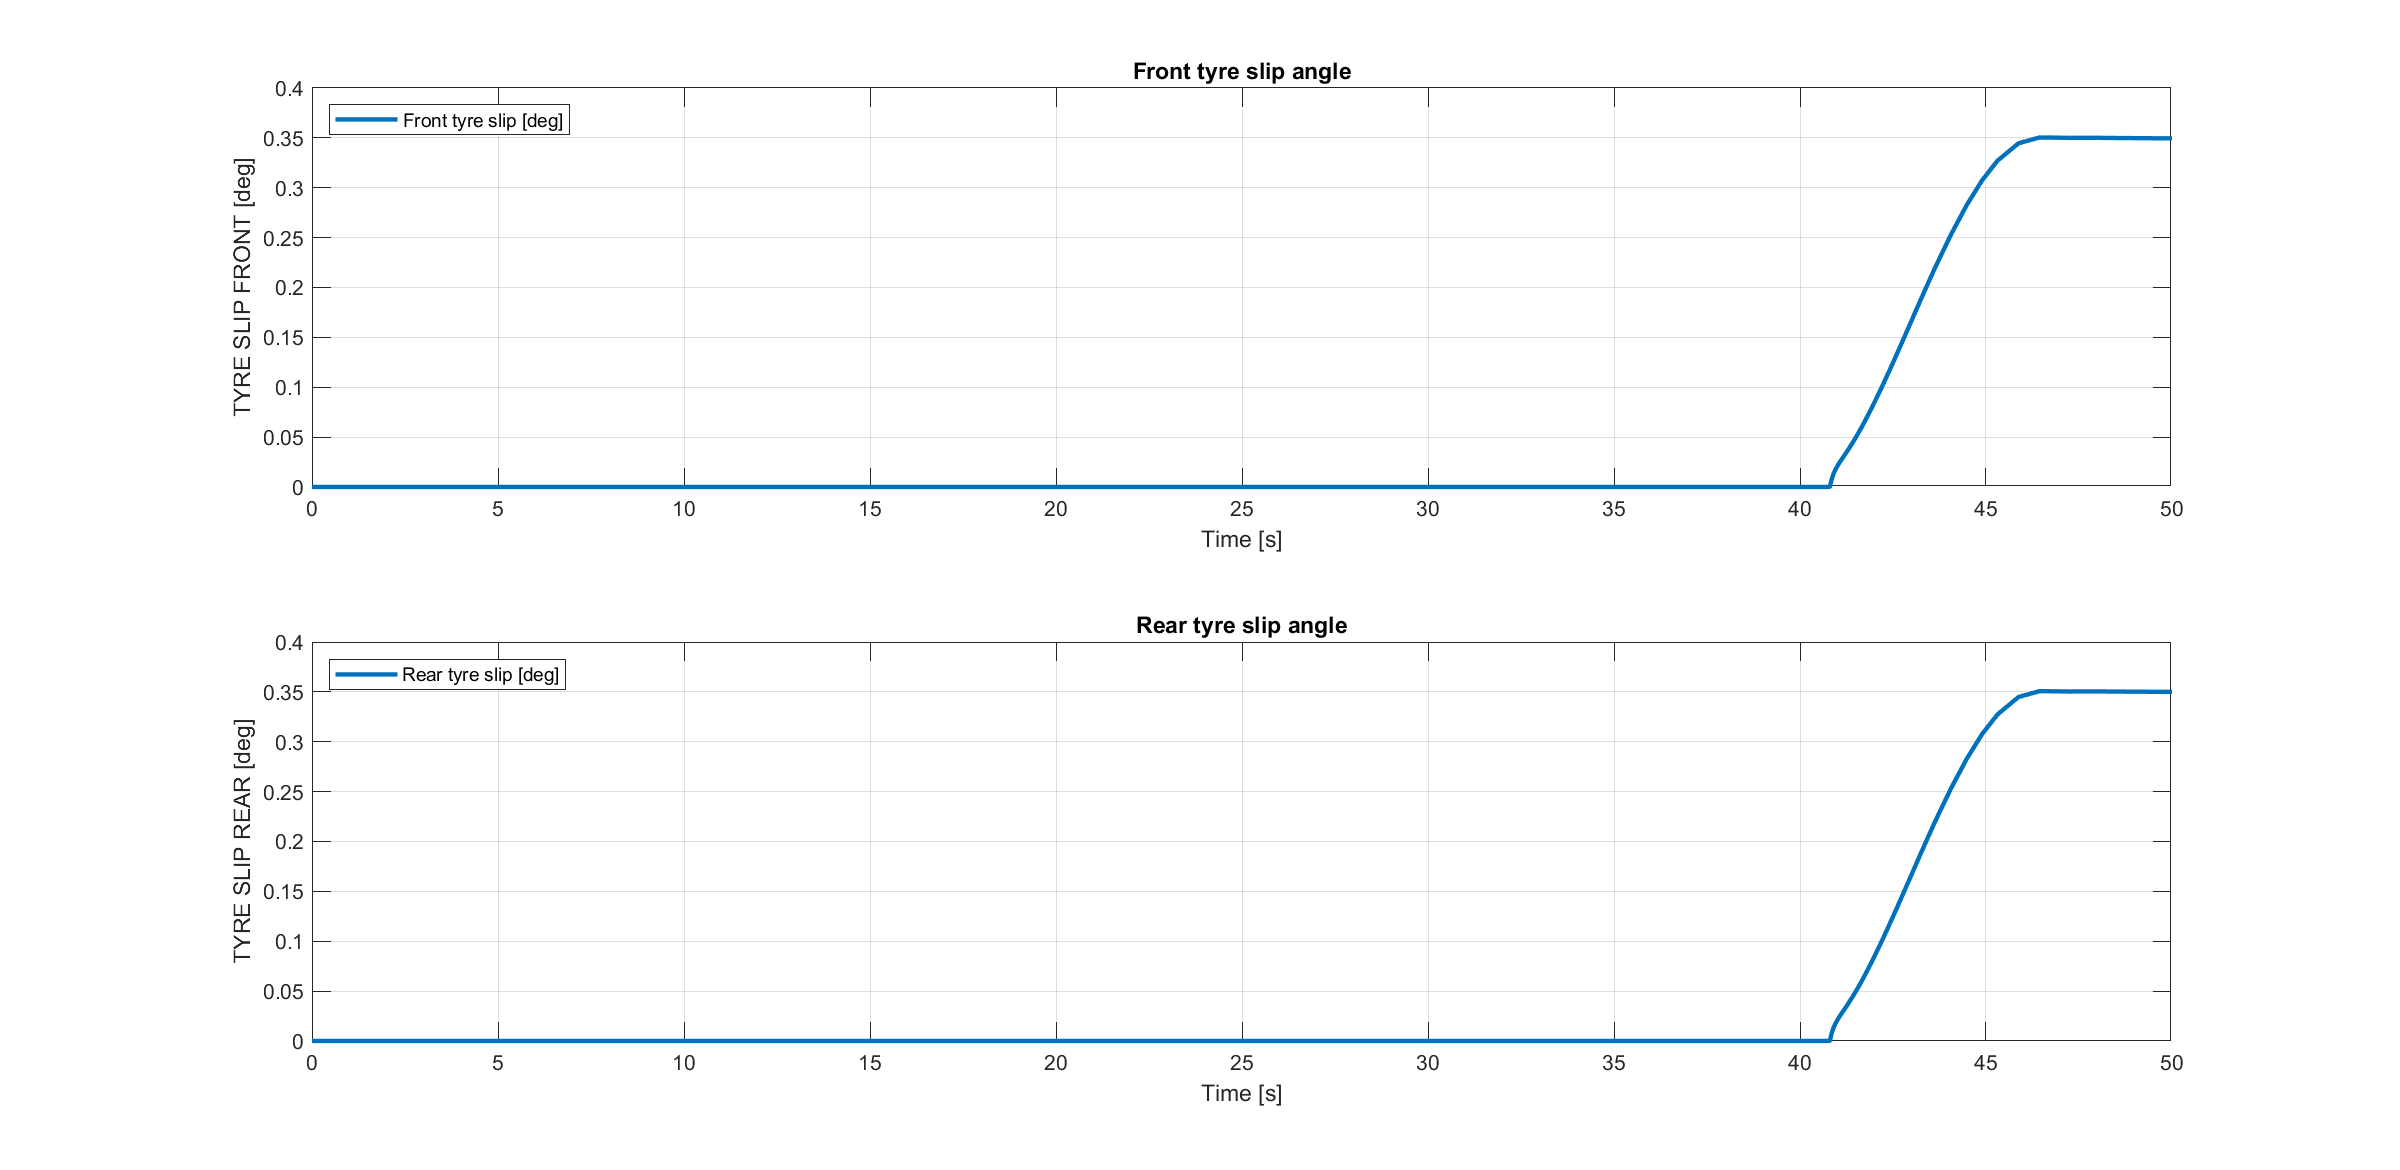
\includegraphics[width=\linewidth]{sim3_slips.png}
    \caption{Simulation 3 - tyre slips figure}
    \label{fig:sim3_4}
\end{figure}

As can be seen, when the ego vehicle starts traversing a banked road about at time 40[s], slip angles, lateral forces and other related figures of merit assume non-zero values. This is clearly consistent with the model dynamics that also takes into account the projection of the vertical load on the inclined road.\\


\subsection{Simulation 4 - Accelerating-Breaking straight path}
In this simulation the aim was to show how the considered figures of merit change when the car is moving on a straight line with positive acceleration and then a braking force is applied to reduce its speed. Provided inputs are: $F_x$ in the form of a step function with $F_x = 1250 [N]$ for $15[s]$, $F_x = -700 [N]$ for the following $15[s]$, $\delta = 0 [rad]$, simulation time = $30 [s]$. Banking is not considered.

\begin{figure}[h!]
    \centering
    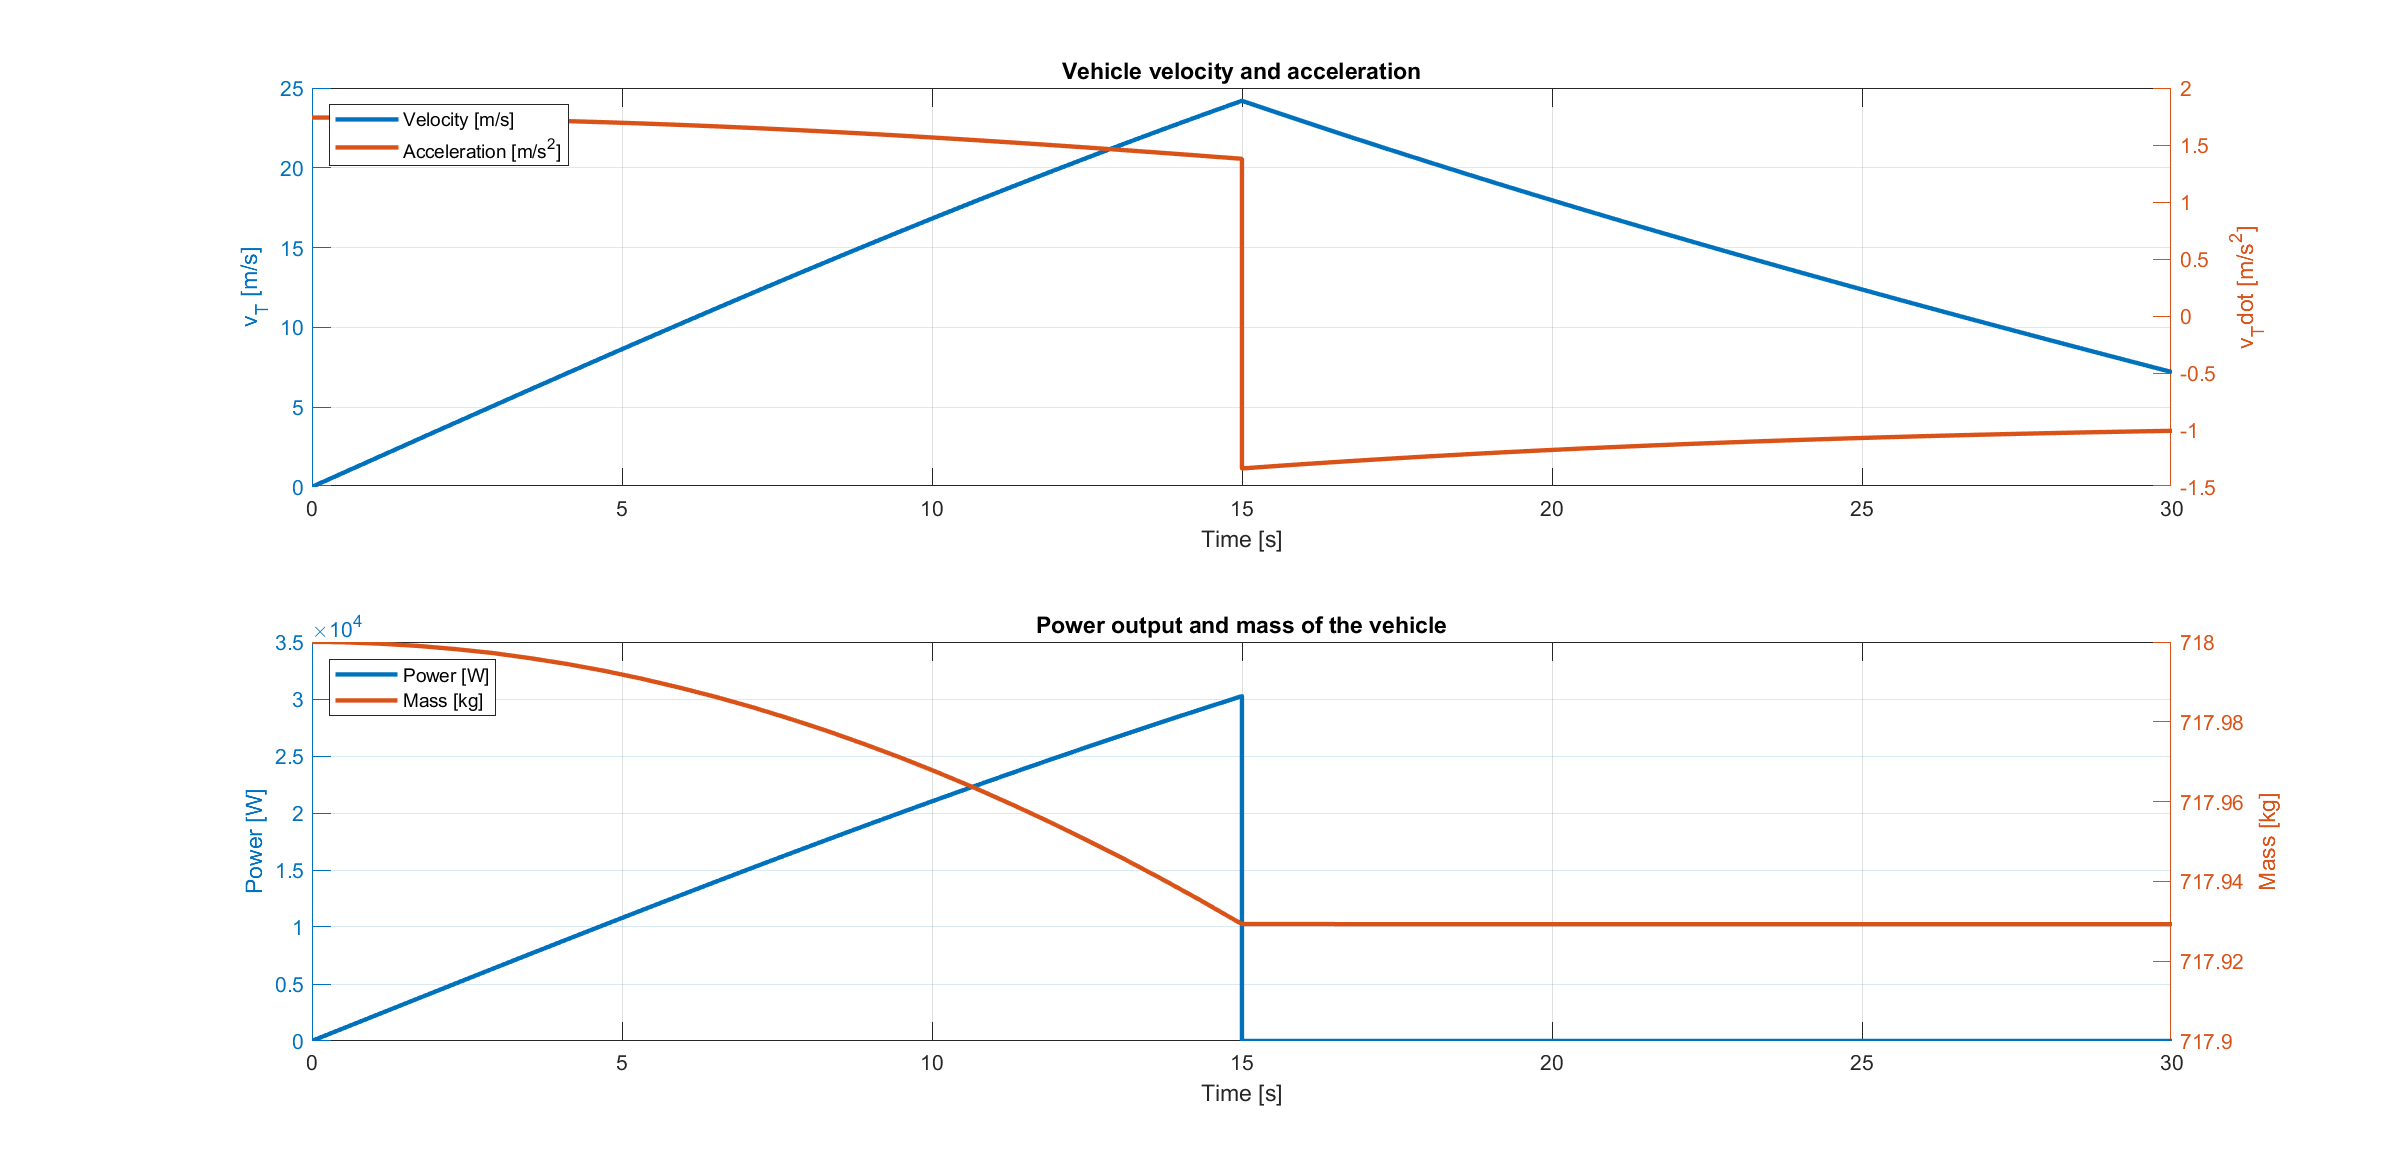
\includegraphics[width=\linewidth]{sim4_vel-power.png}
    \caption{Simulation 4 - velocity, acceleration, power and mass figure}
    \label{fig:sim4_1}
\end{figure}

\begin{figure}[h!]
    \centering
    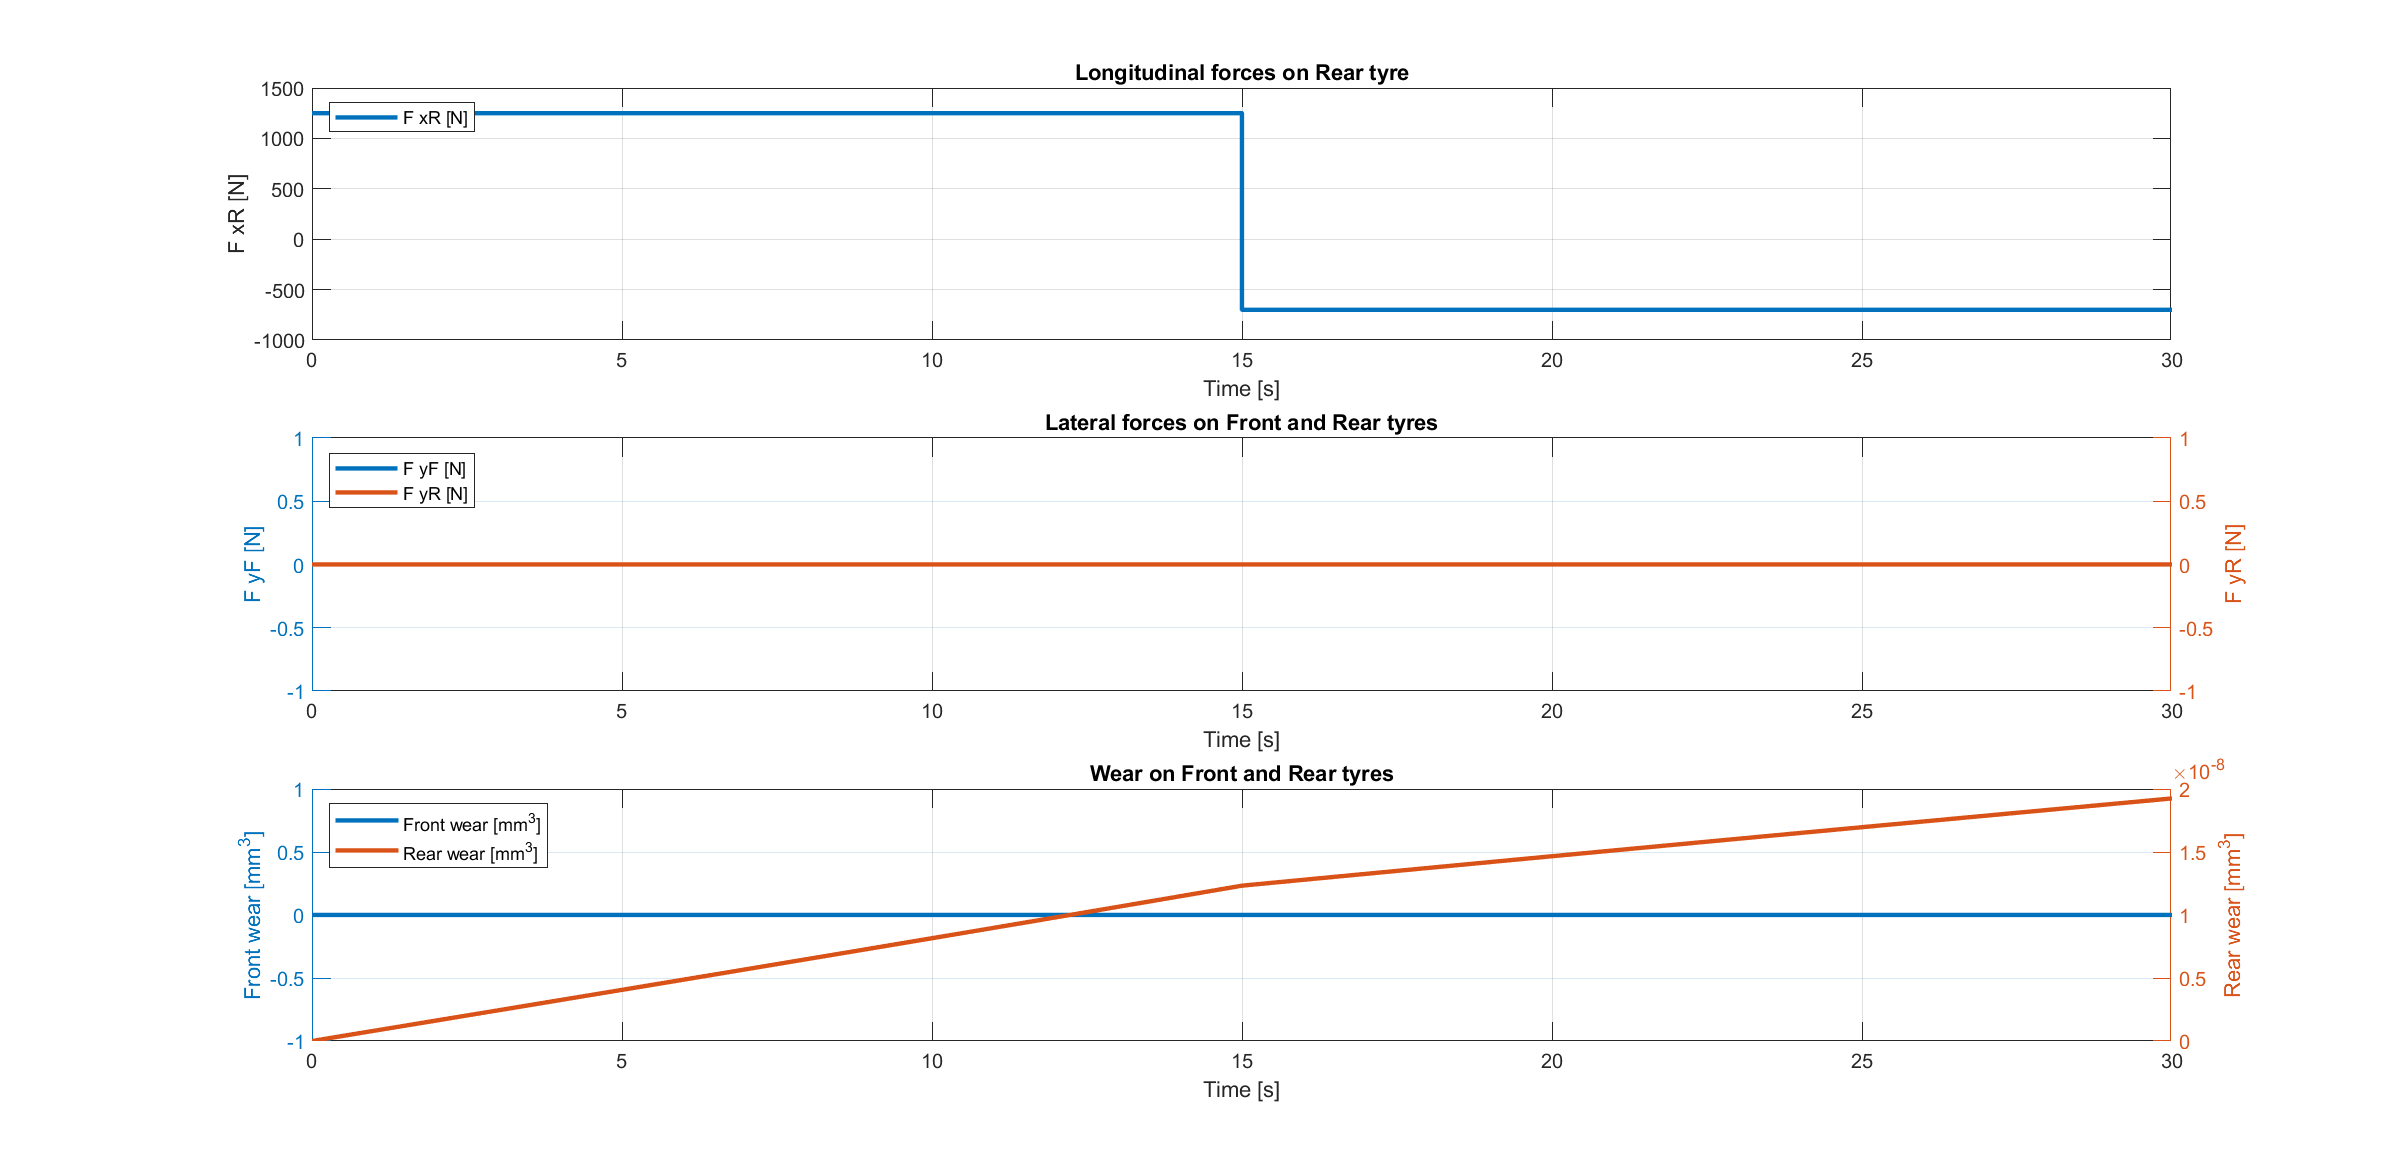
\includegraphics[width=\linewidth]{sim4_force-wear.png}
    \caption{Simulation 4 - forces and tyres wear figure}
    \label{fig:sim4_2}
\end{figure}

In this simulation the images related to the figures of merit such as trajectory, slip angle and yaw angles are omitted because always keep a zero value. The shown images are consistent with the vehicle dynamics: as we can see the velocity increases as far as $F_x$ is positive and starts decreasing in the second half of the simulation when $F_x$ holds a negative value. Another important aspect that can be highlighted is the model of the fuel tank that is coherent with the shown results: when the input force $F_x$ has negative values the power produced by the vehicle is considered null as well as the fuel consumption.\\

\subsection{Simulation 5 - Constant steer and increasing velocity path}
The aim of simulation 5 was to test the correctness of the various figures of merit in a "circle trajectory" situation with increasing velocity. The car starts with an initial speed of $0[m/s]$ and then constantly accelerates and steers to the left. Provided inputs are $F_x = 1500 [N]$, $\delta = 0 [rad]$ for the first $0.5[s]$ and then constantly increases up to about $0.03 [rad]$, simulation time = $45 [s]$.
\\In this case the shown figures represent the trajectory, the angles and the lateral forces. As can be seen, the yaw angle constantly increases, since the vehicle is constantly turning, and up to a certain time point also the yaw rate is increasing before settling down. Also lateral forces have a positive growth since it is a left-turning manoeuvre.\\ 
\begin{figure}[h!]
    \centering
    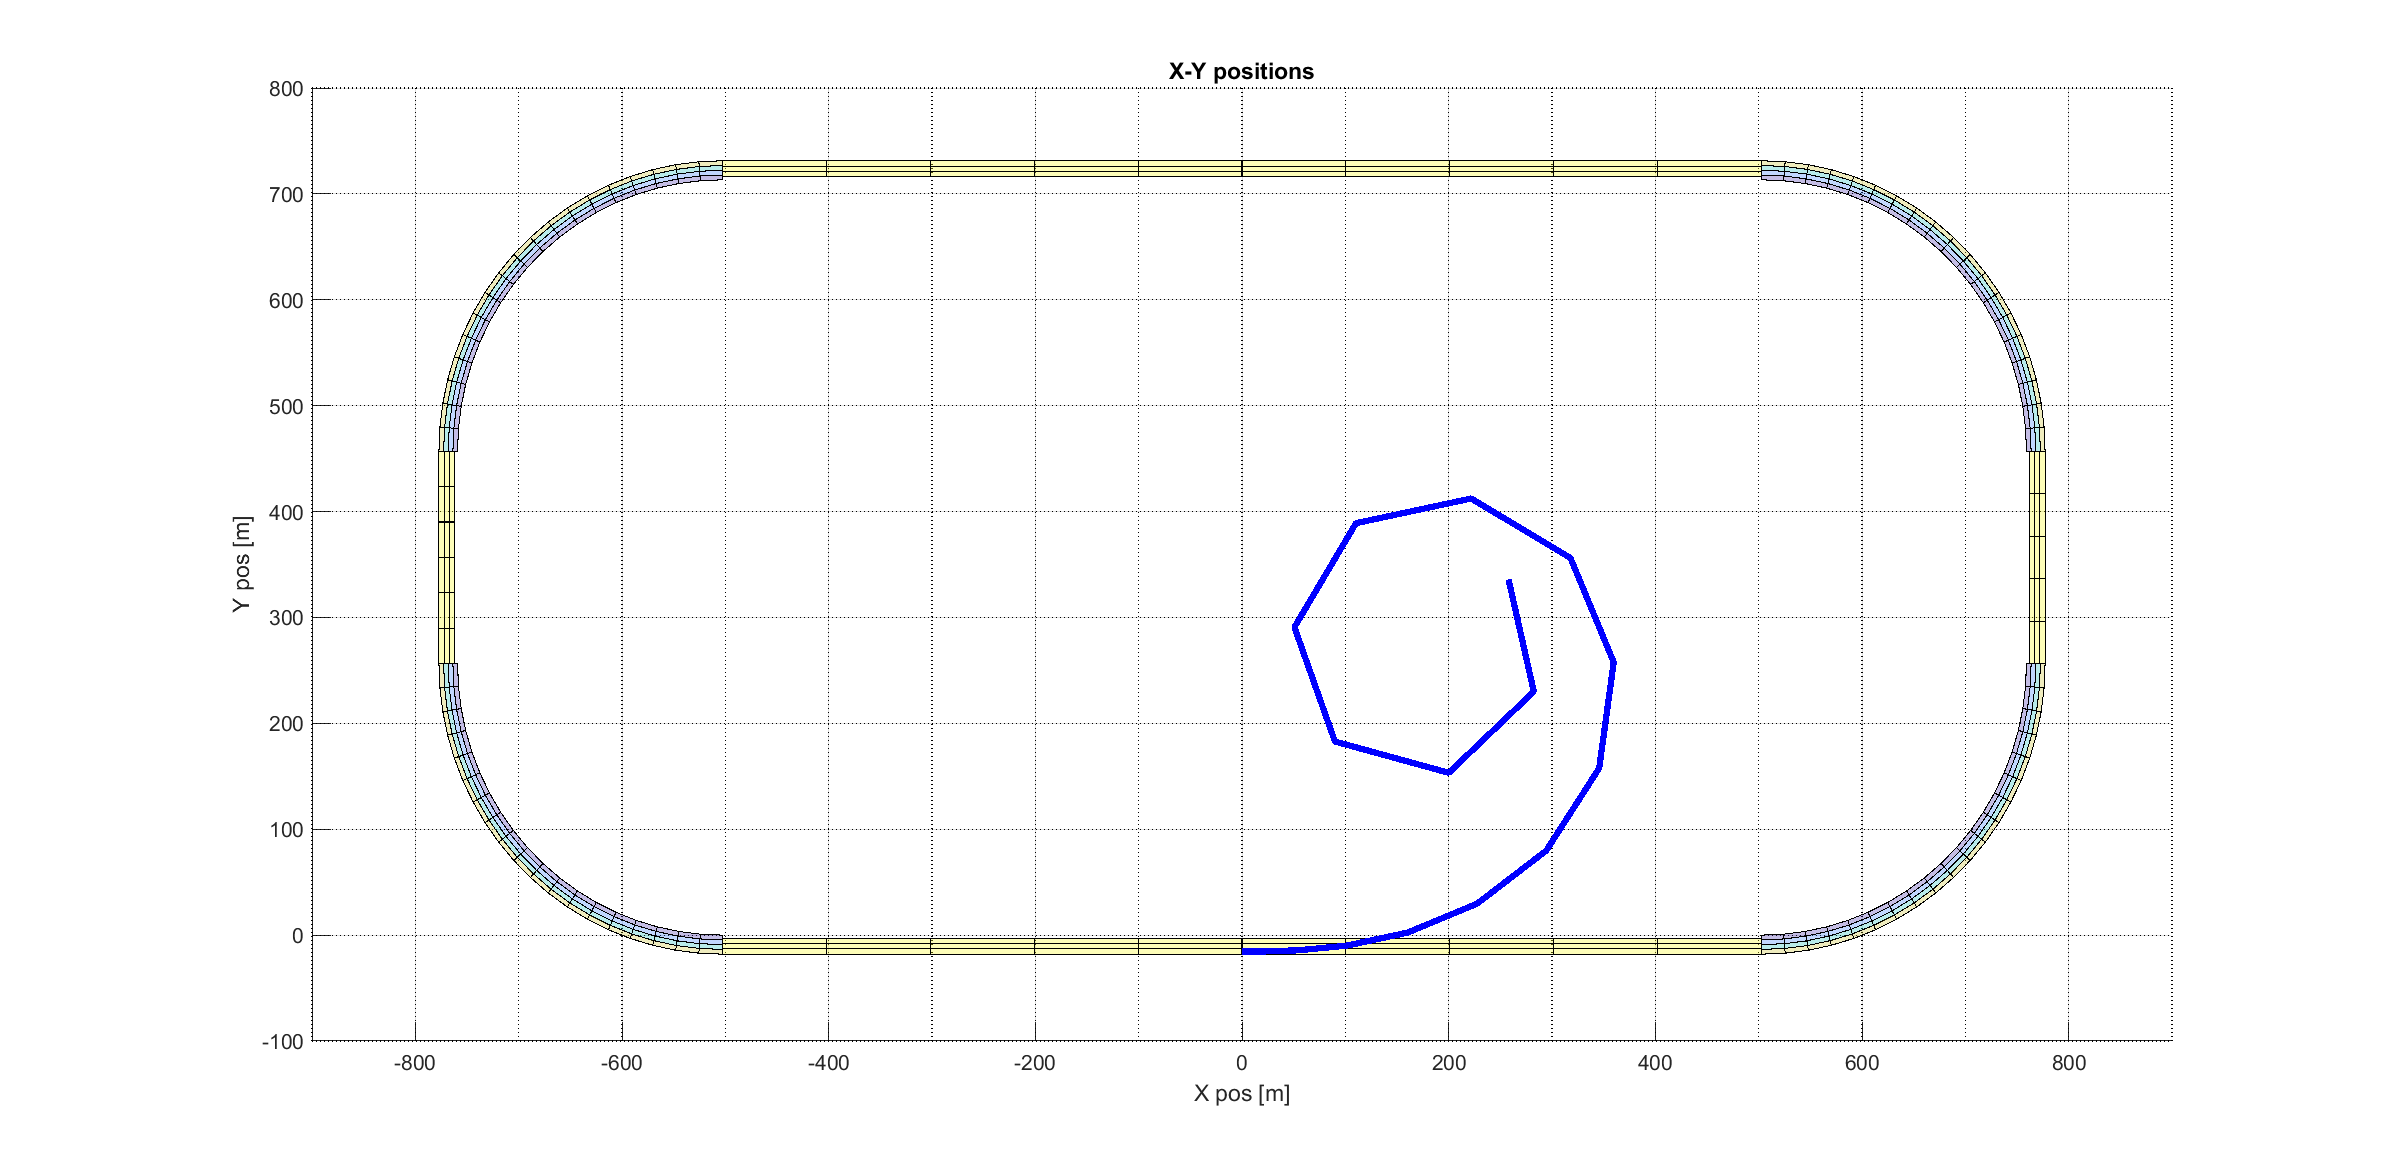
\includegraphics[width=\linewidth]{sim5_trajectory.png}
    \caption{Simulation 5 - trajectory of the vehicle}
    \label{fig:sim5_1}
\end{figure}
\begin{figure}[h!]
    \centering
    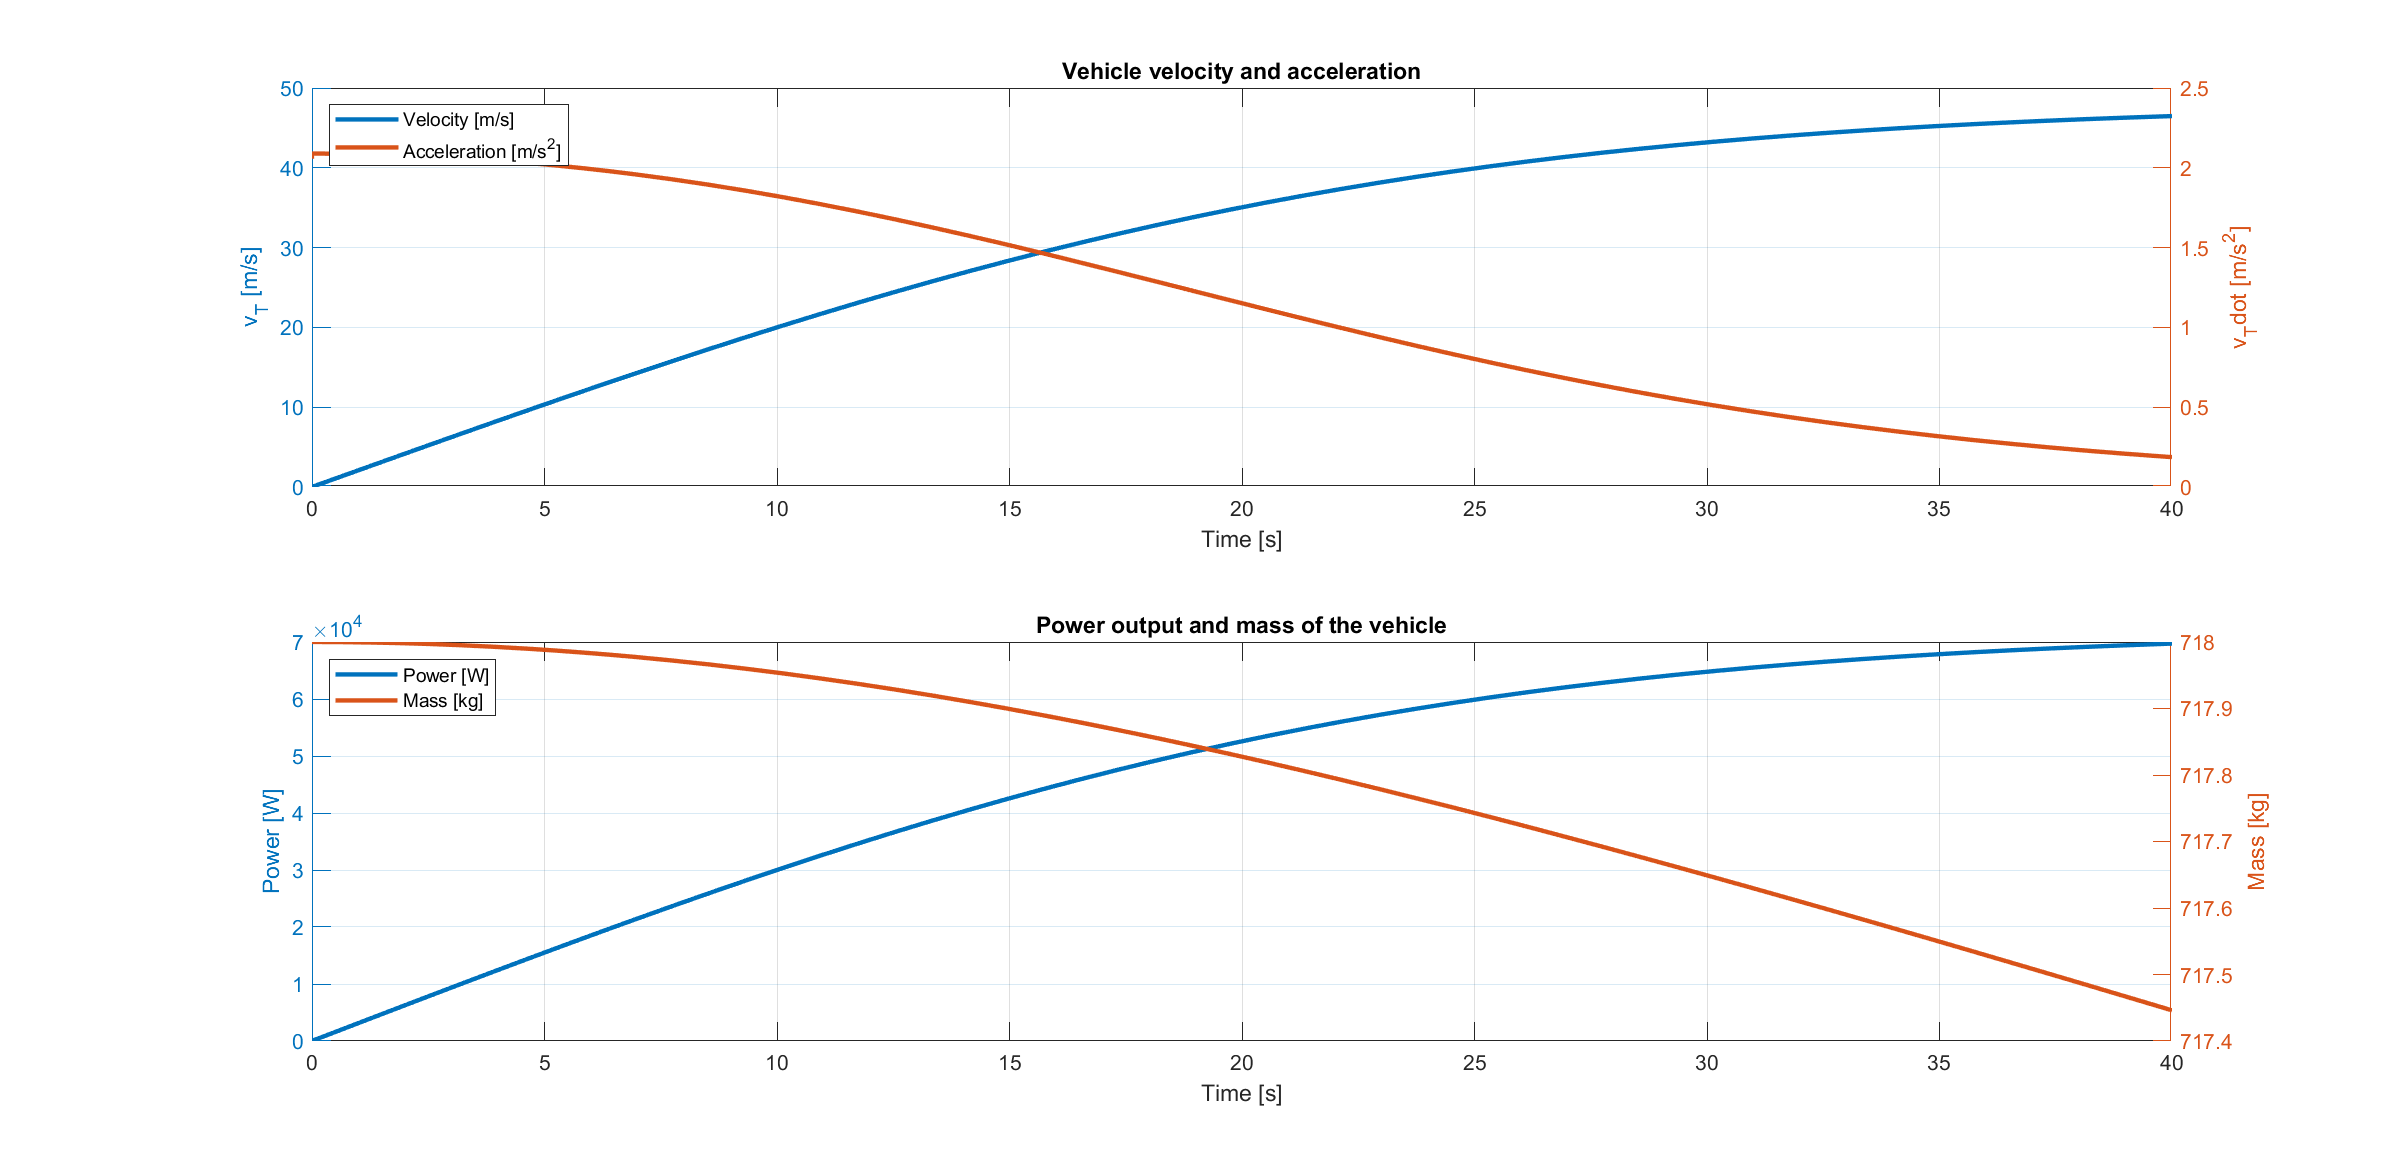
\includegraphics[width=\linewidth]{sim5_vel-power.png}
    \caption{Simulation 5 - velocity, acceleration, power and mass figure}
    \label{fig:sim5_2}
\end{figure}
\begin{figure}[h!]
    \centering
    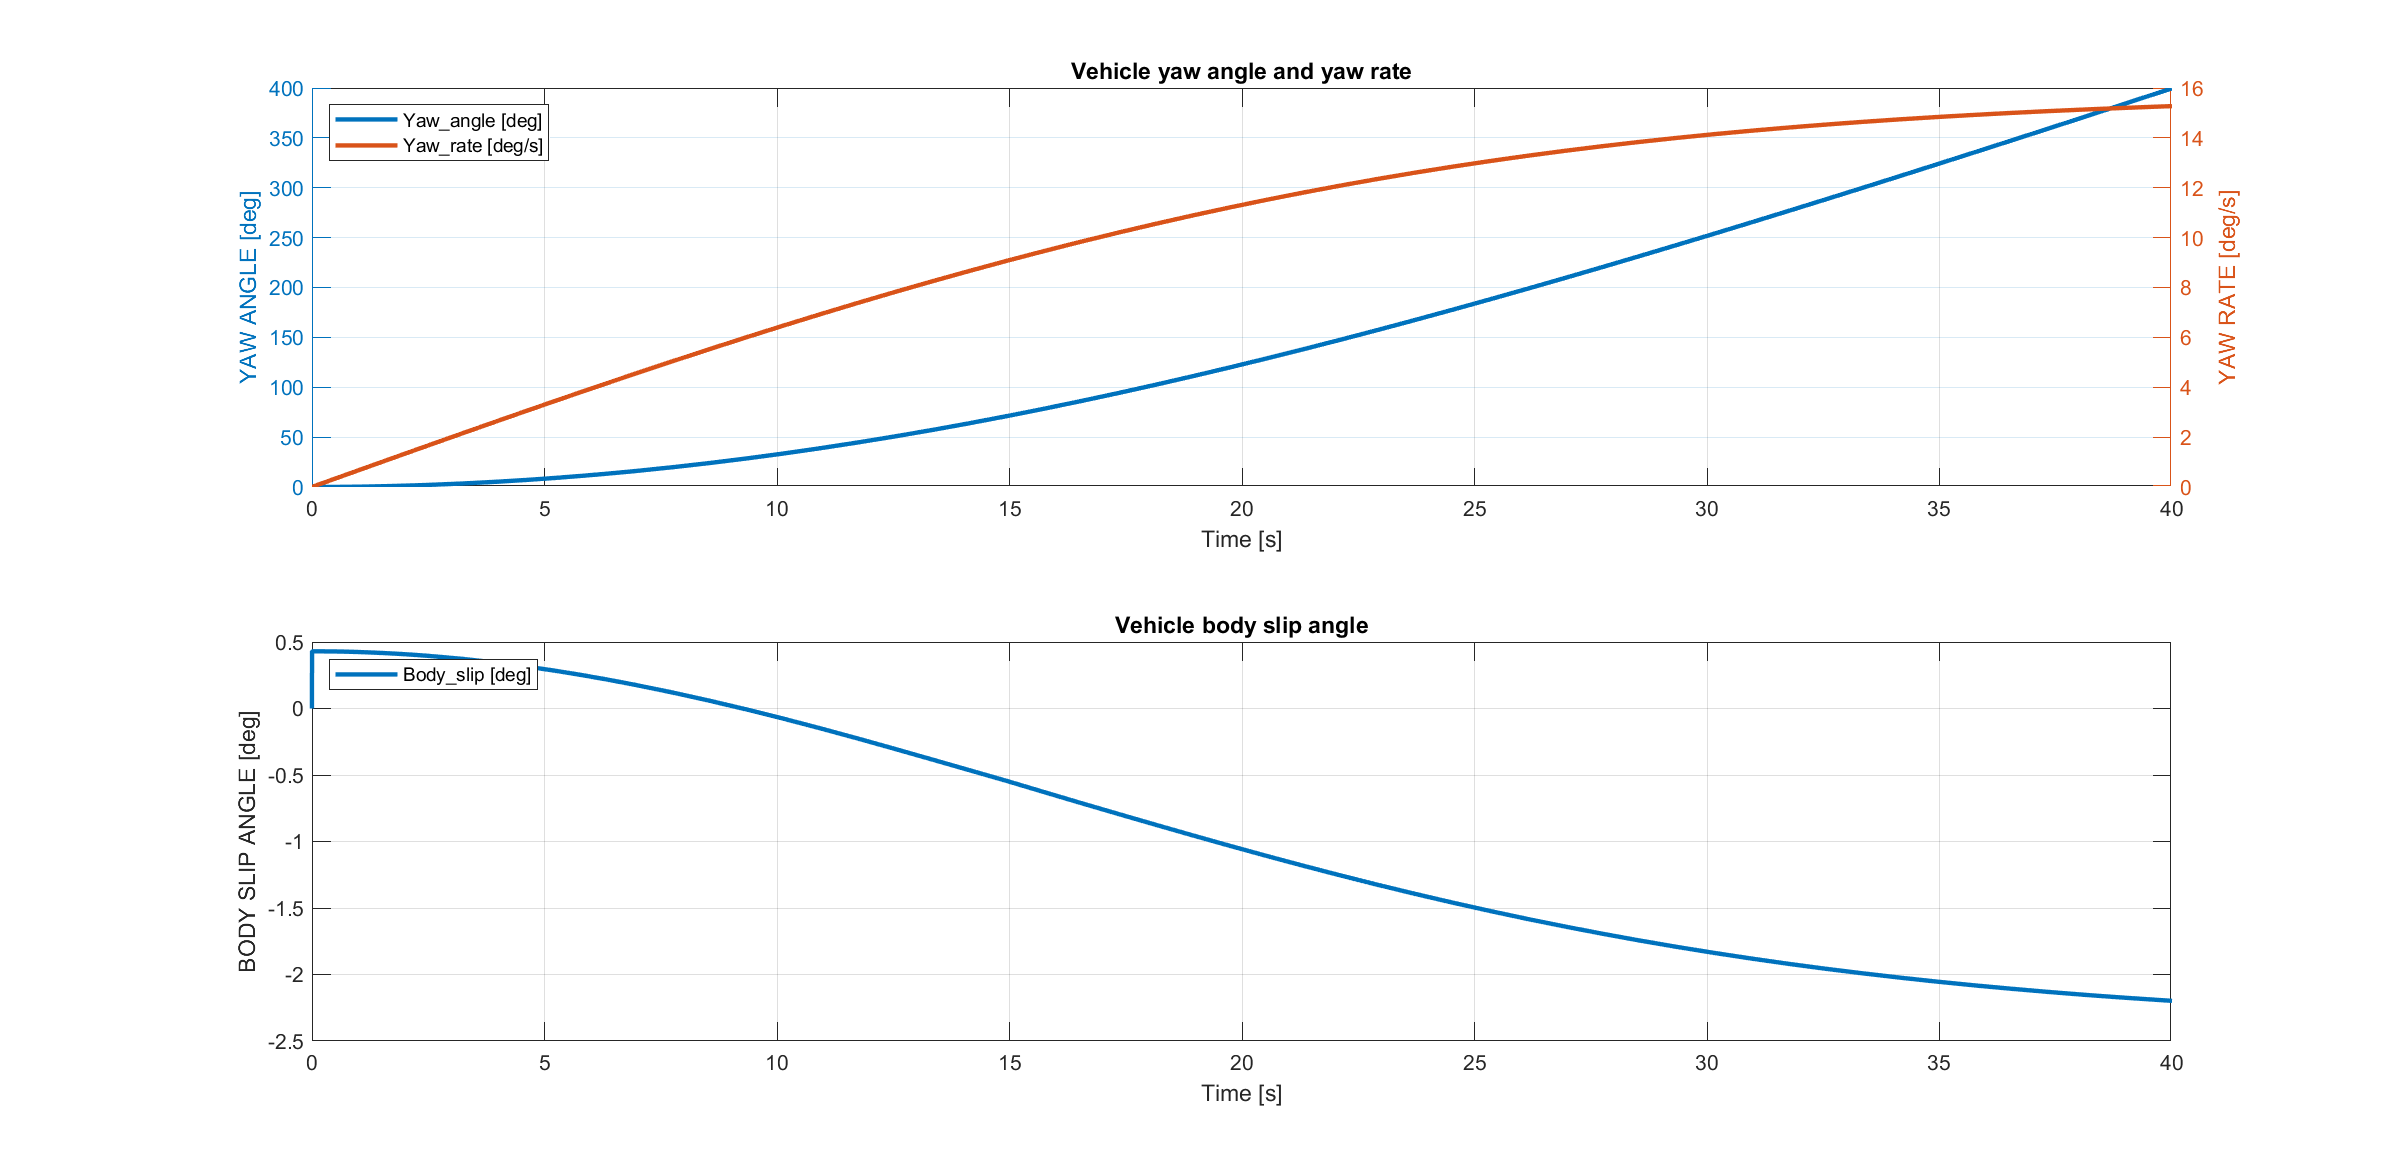
\includegraphics[width=\linewidth]{sim5_angles.png}
    \caption{Simulation 5 - angles figure}
    \label{fig:sim5_3}
\end{figure}
\begin{figure}[h!]
    \centering
    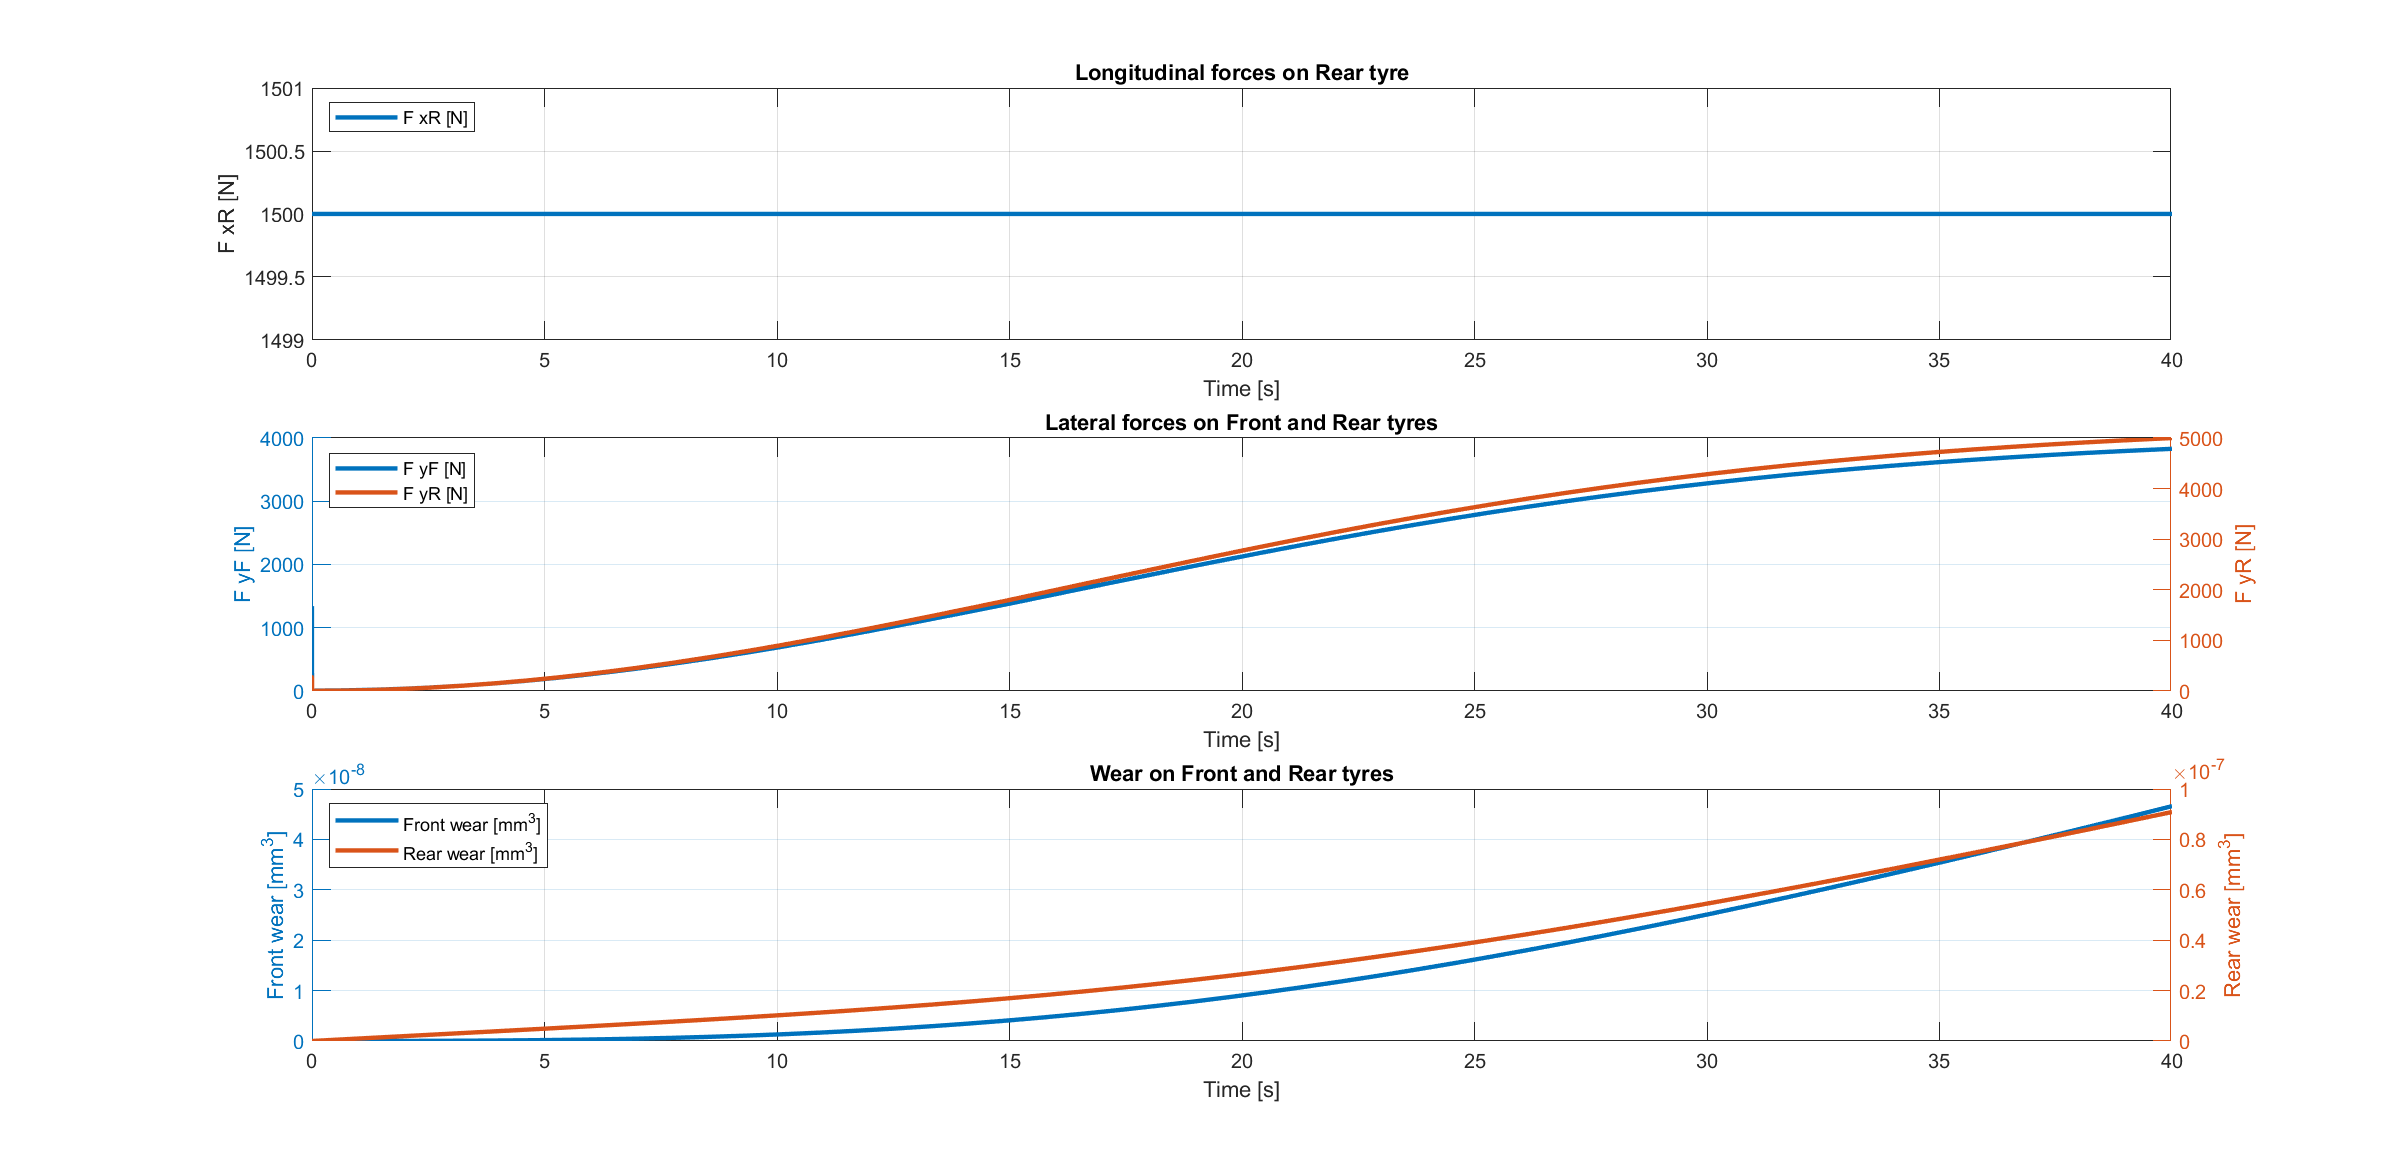
\includegraphics[width=\linewidth]{sim5_force-wear.png}
    \caption{Simulation 5 - forces and tyres wear figure}
    \label{fig:sim5_4}
\end{figure}

\subsection{Simulation 6 - Sinusoidal wave path}
The aim of this simulation was to test the correctness of the various figures of merit in a "sinusoidal wave trajectory" situation. The car starts with an initial speed of $0[m/s]$ and then constantly accelerates and steers following a sinusoidal wave with amplitude about $0.02[rad]$ and frequency $0.22[rad/s]$. Provided inputs are $F_x = 500 [N]$, $\delta = 0.02sin(0.22t)$, simulation time = $30 [s]$. \\For the given simulation time and frequency, just a single wave is simulated. The shown figures represent the trajectory, the angles and the lateral forces. Power and mass figures are not shown since consistent with simulation scenario and already shown in previous simulations. All the figures provided exhibit a wave behavior consistent with the simulation data.  
\begin{figure}[h!]
    \centering
    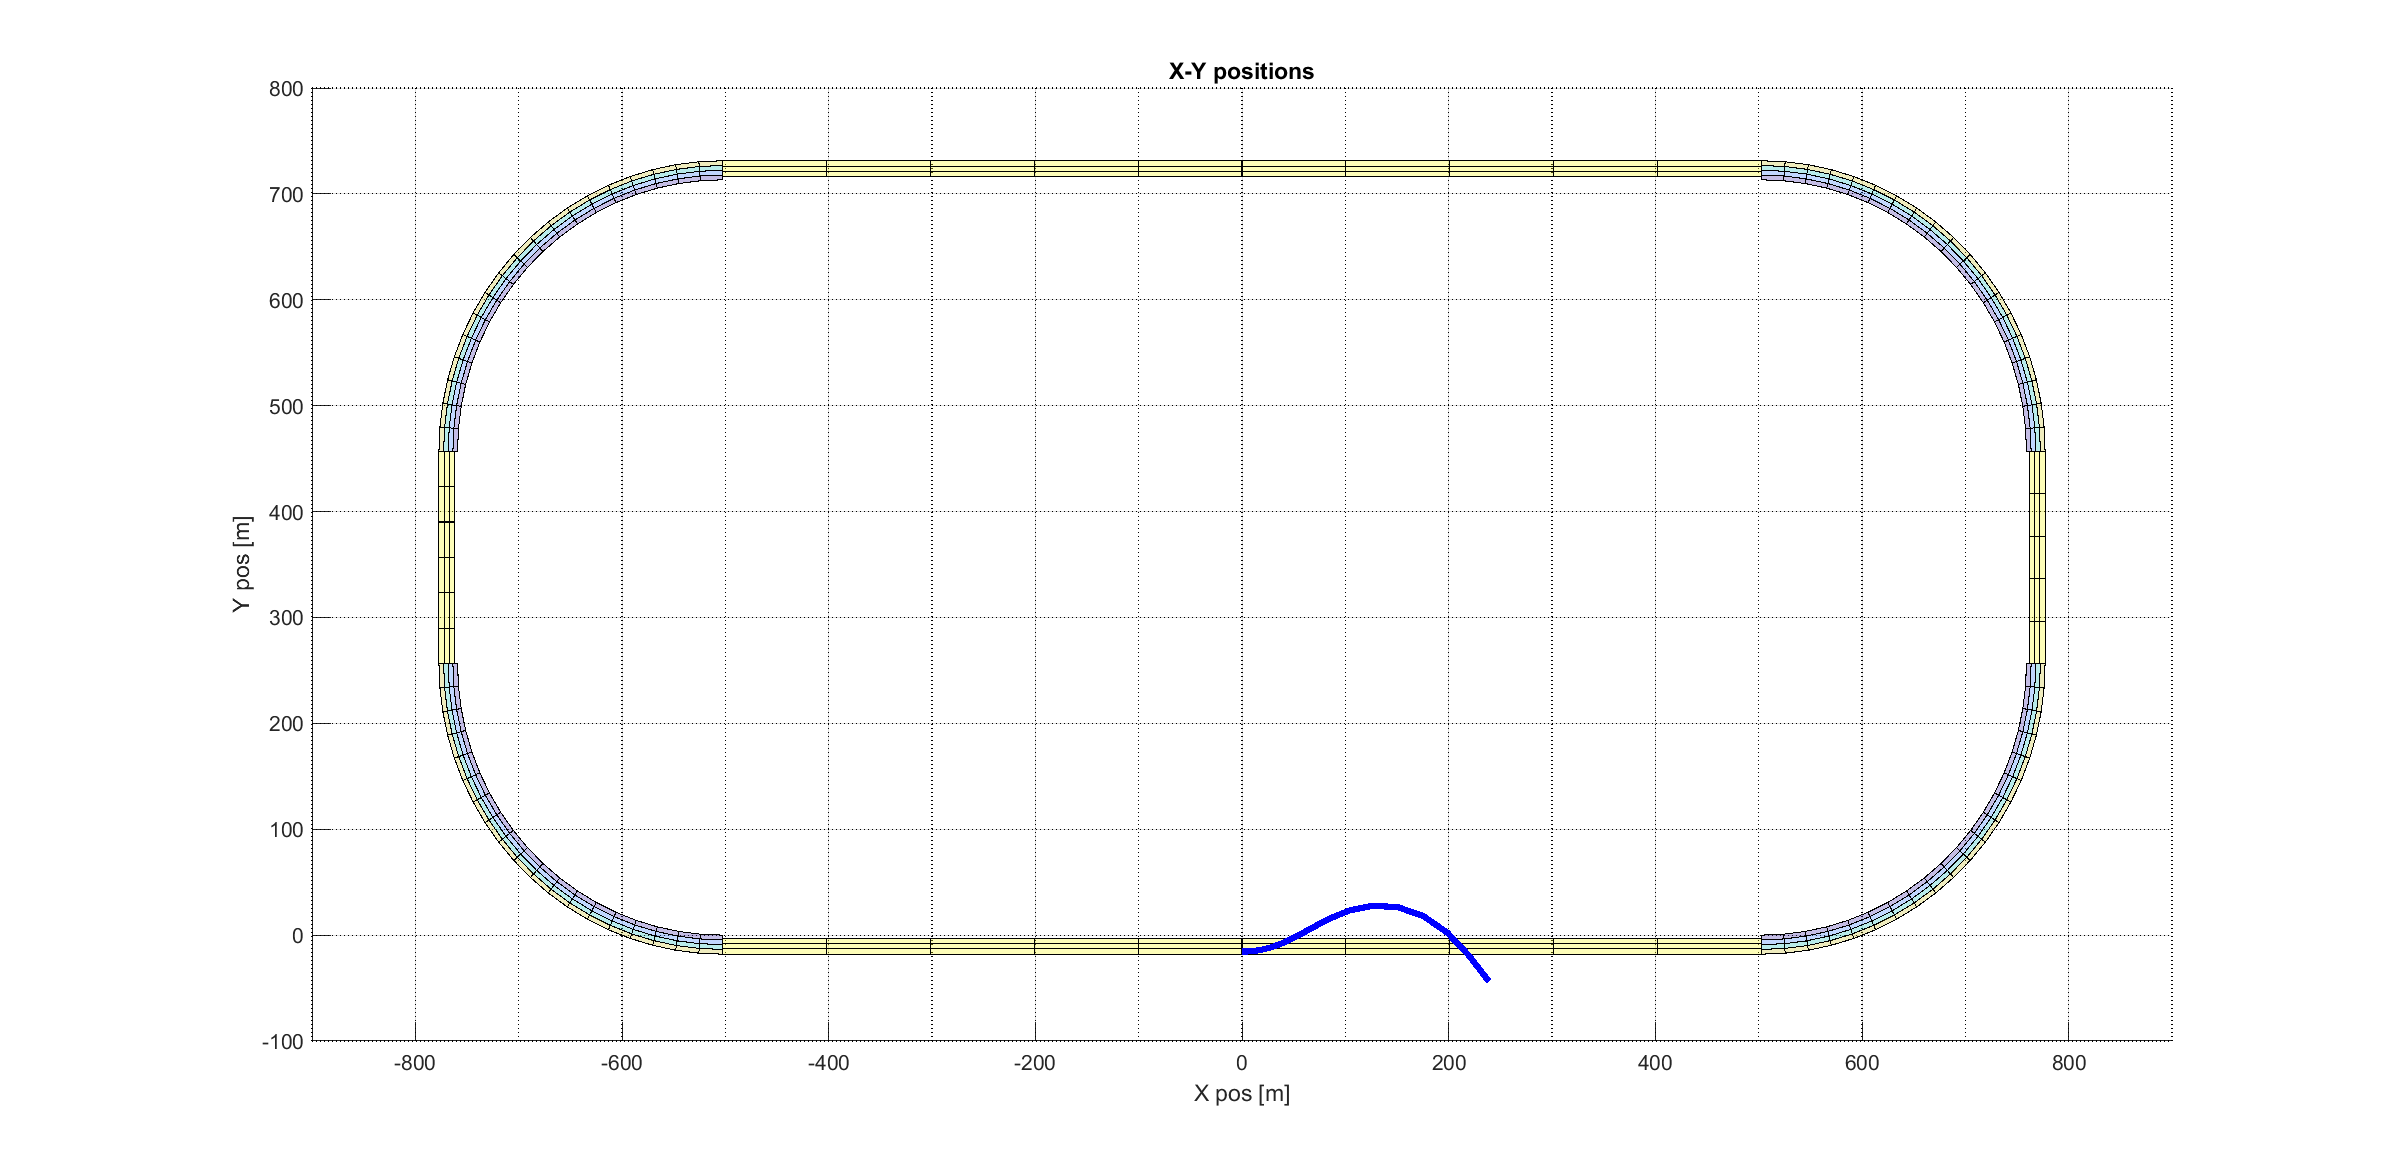
\includegraphics[width=\linewidth]{sim6_trajectory.png}
    \caption{Simulation 6 - trajectory of the vehicle}
    \label{fig:sim6_1}
\end{figure}
\begin{figure}[h!]
    \centering
    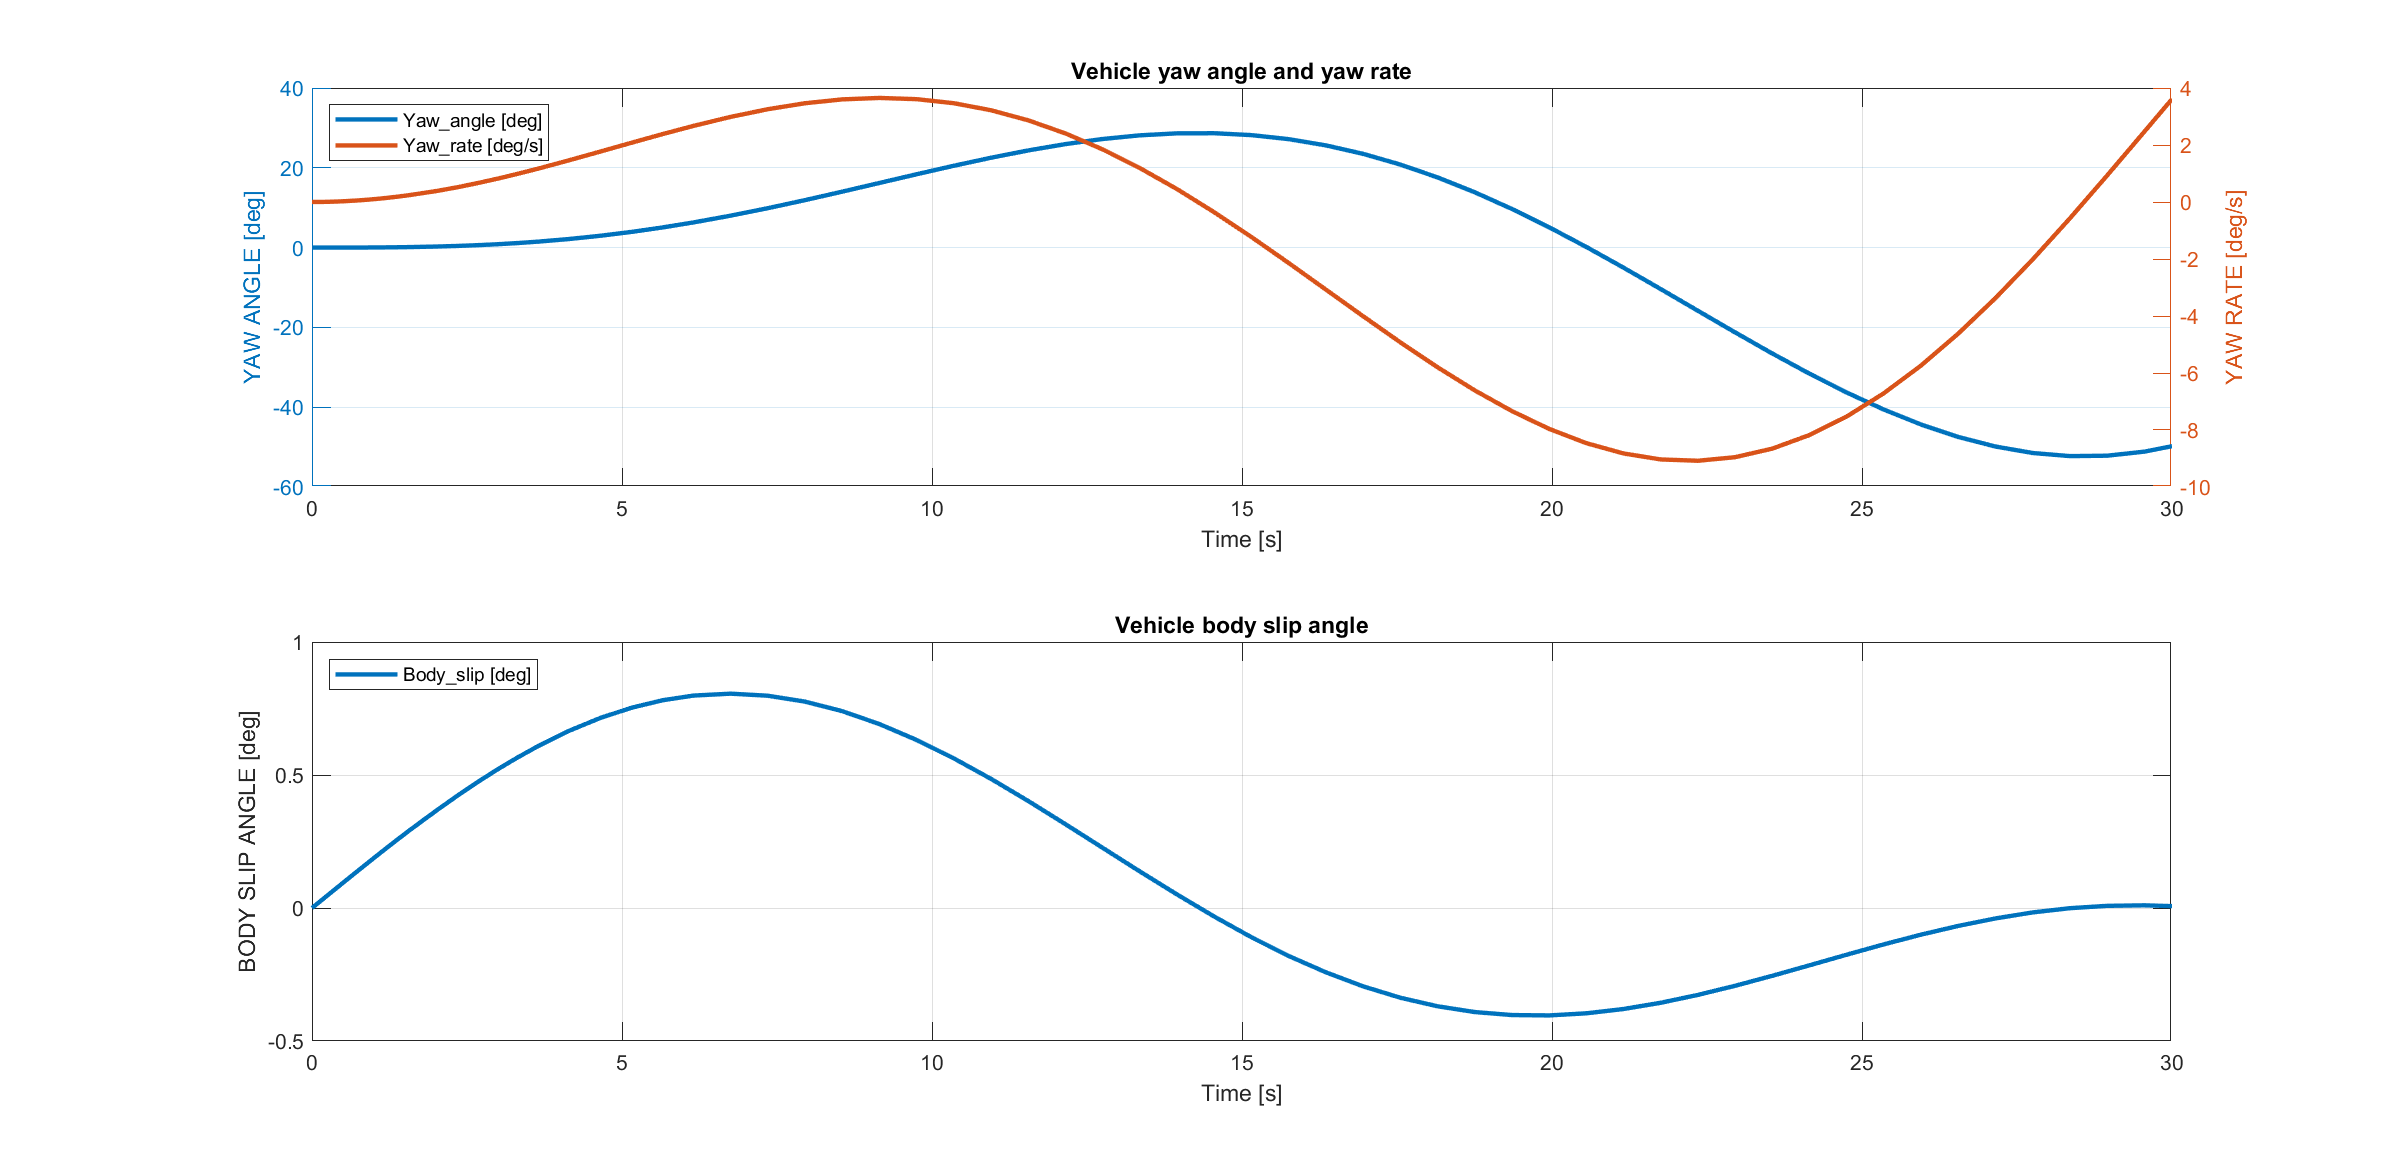
\includegraphics[width=\linewidth]{sim6_angles.png}
    \caption{Simulation 6 - angles figure}
    \label{fig:sim6_2}
\end{figure}
\begin{figure}[h!]
    \centering
    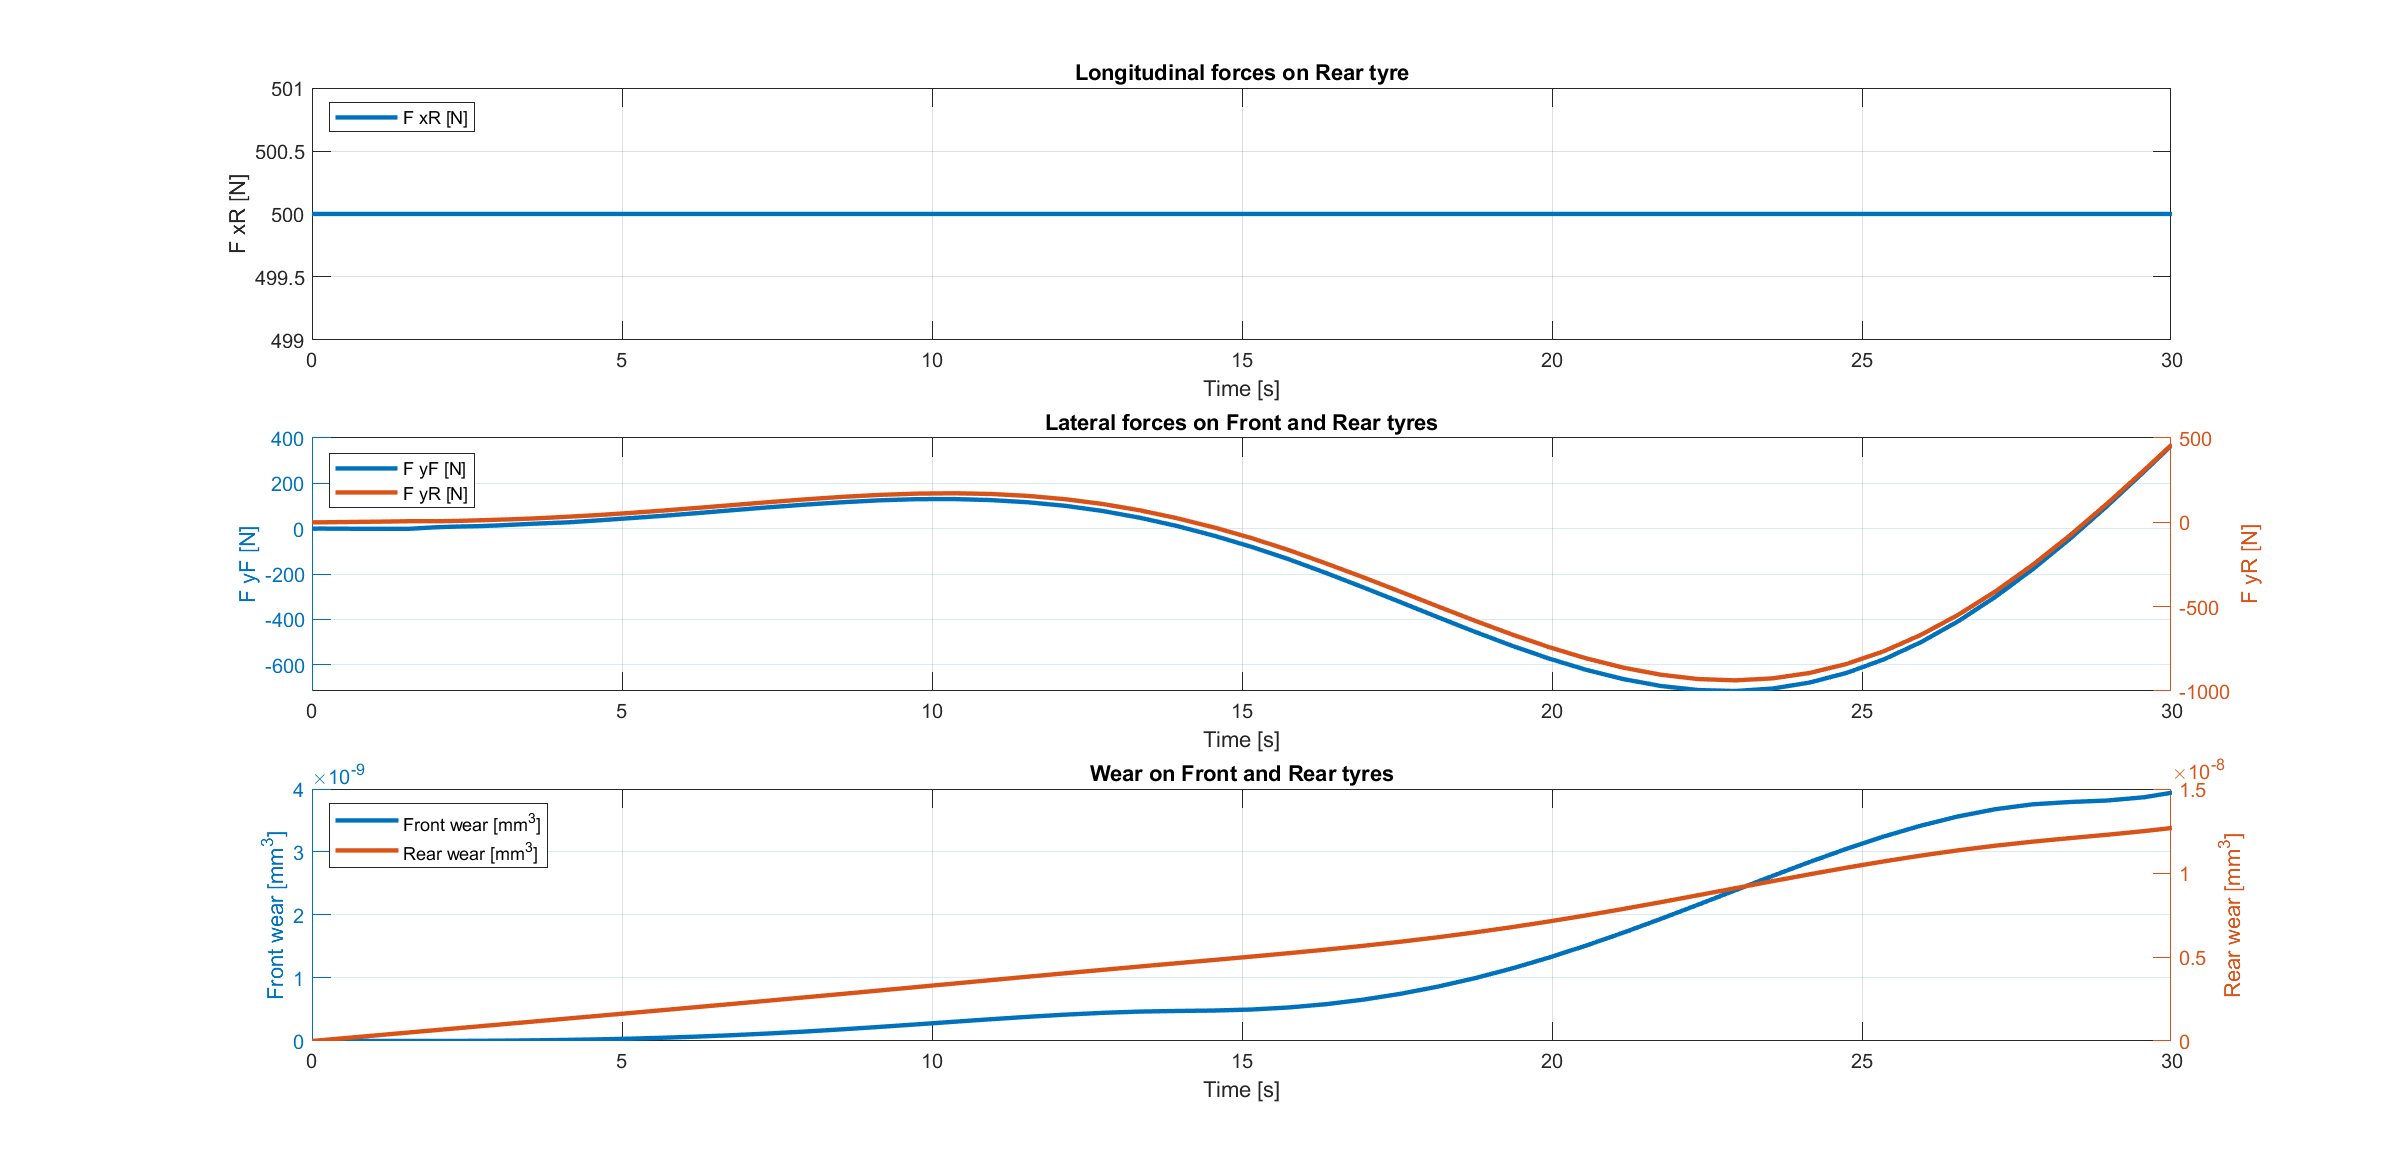
\includegraphics[width=\linewidth]{sim6_force-wear.png}
    \caption{Simulation 6 - forces and tyres wear figure}
    \label{fig:sim6_3}
\end{figure}


\subsection{Simulation 7 - Constant speed and increasing steering angle}
The aim of this simulation was to test the correctness of the various figures of merit in a sort of circular trajectory with a constant speed. The car starts with a speed of $30[m/s]$ and after few seconds reaches its desired speed of $50[m/s]$ speed. The applied steering angle is a linear function with slope of $3[deg/s]$ and the simulation is run for $100[s]$: this will result in a final steering angle on the wheels of $30[deg/s]$. The velocity is kept constant by using a simple PID controller. As it is clear also from the figure representing the trajectory, the presented vehicle shows an under-steering behaviour because it enlarges the trajectory even if the applied steering angle is increasing. 
\begin{figure}[h!]
    \centering
    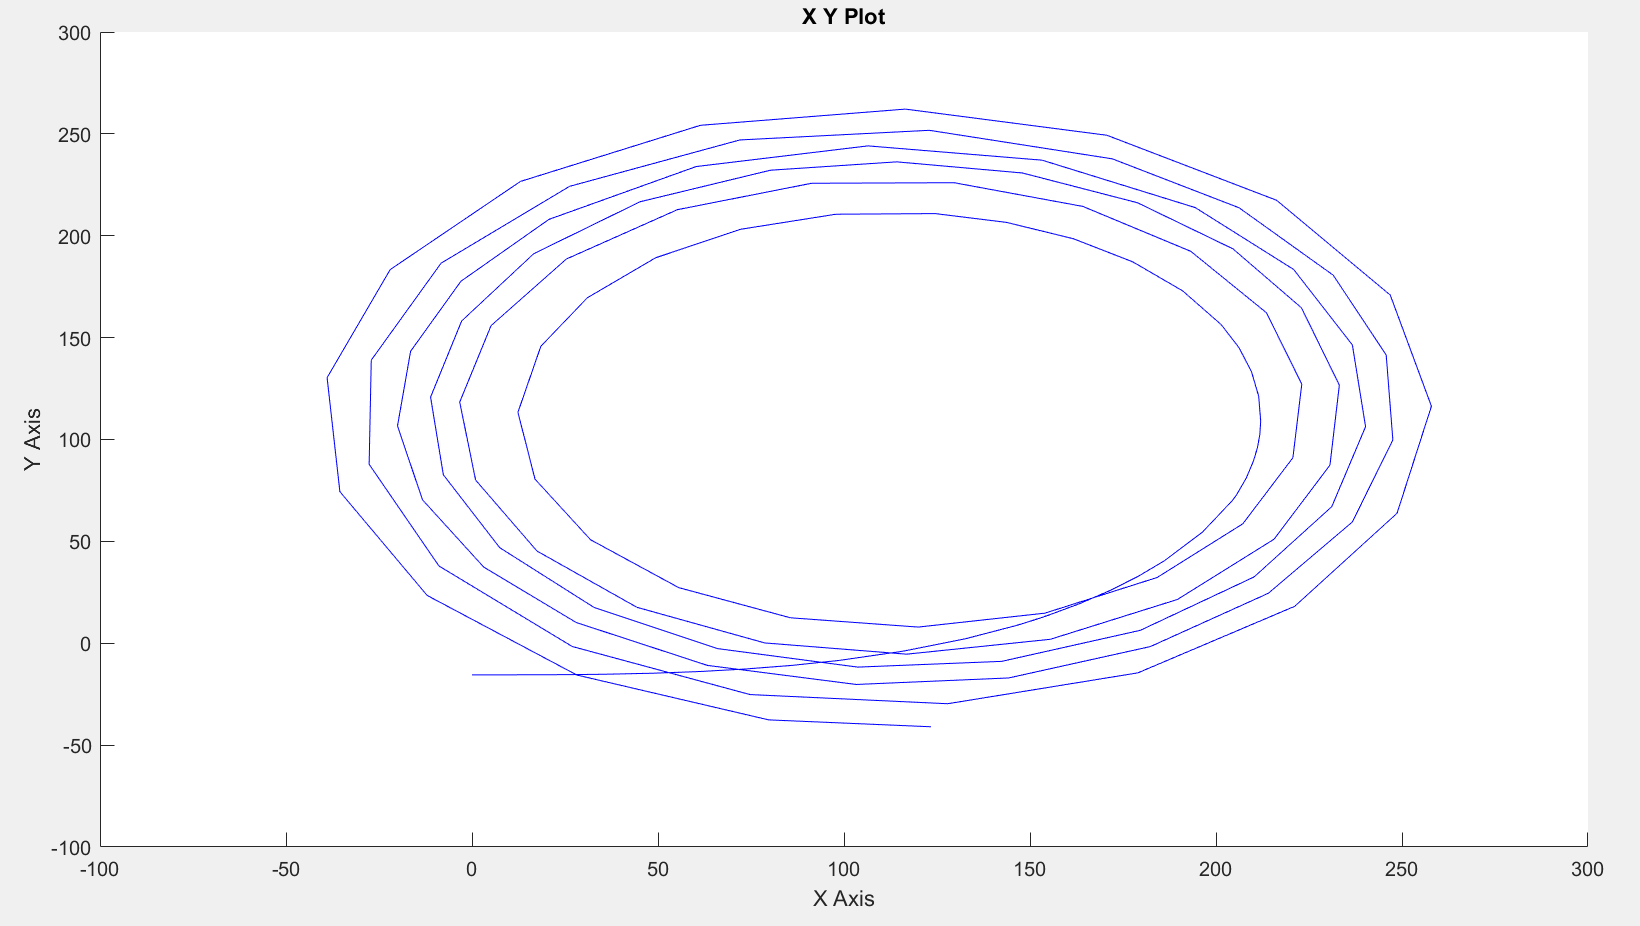
\includegraphics[width=\linewidth]{sim7_trajectory2.png}
    \caption{Simulation 7 - trajectory of the vehicle}
    \label{fig:sim6_1}
\end{figure}
\begin{figure}[h!]
    \centering
    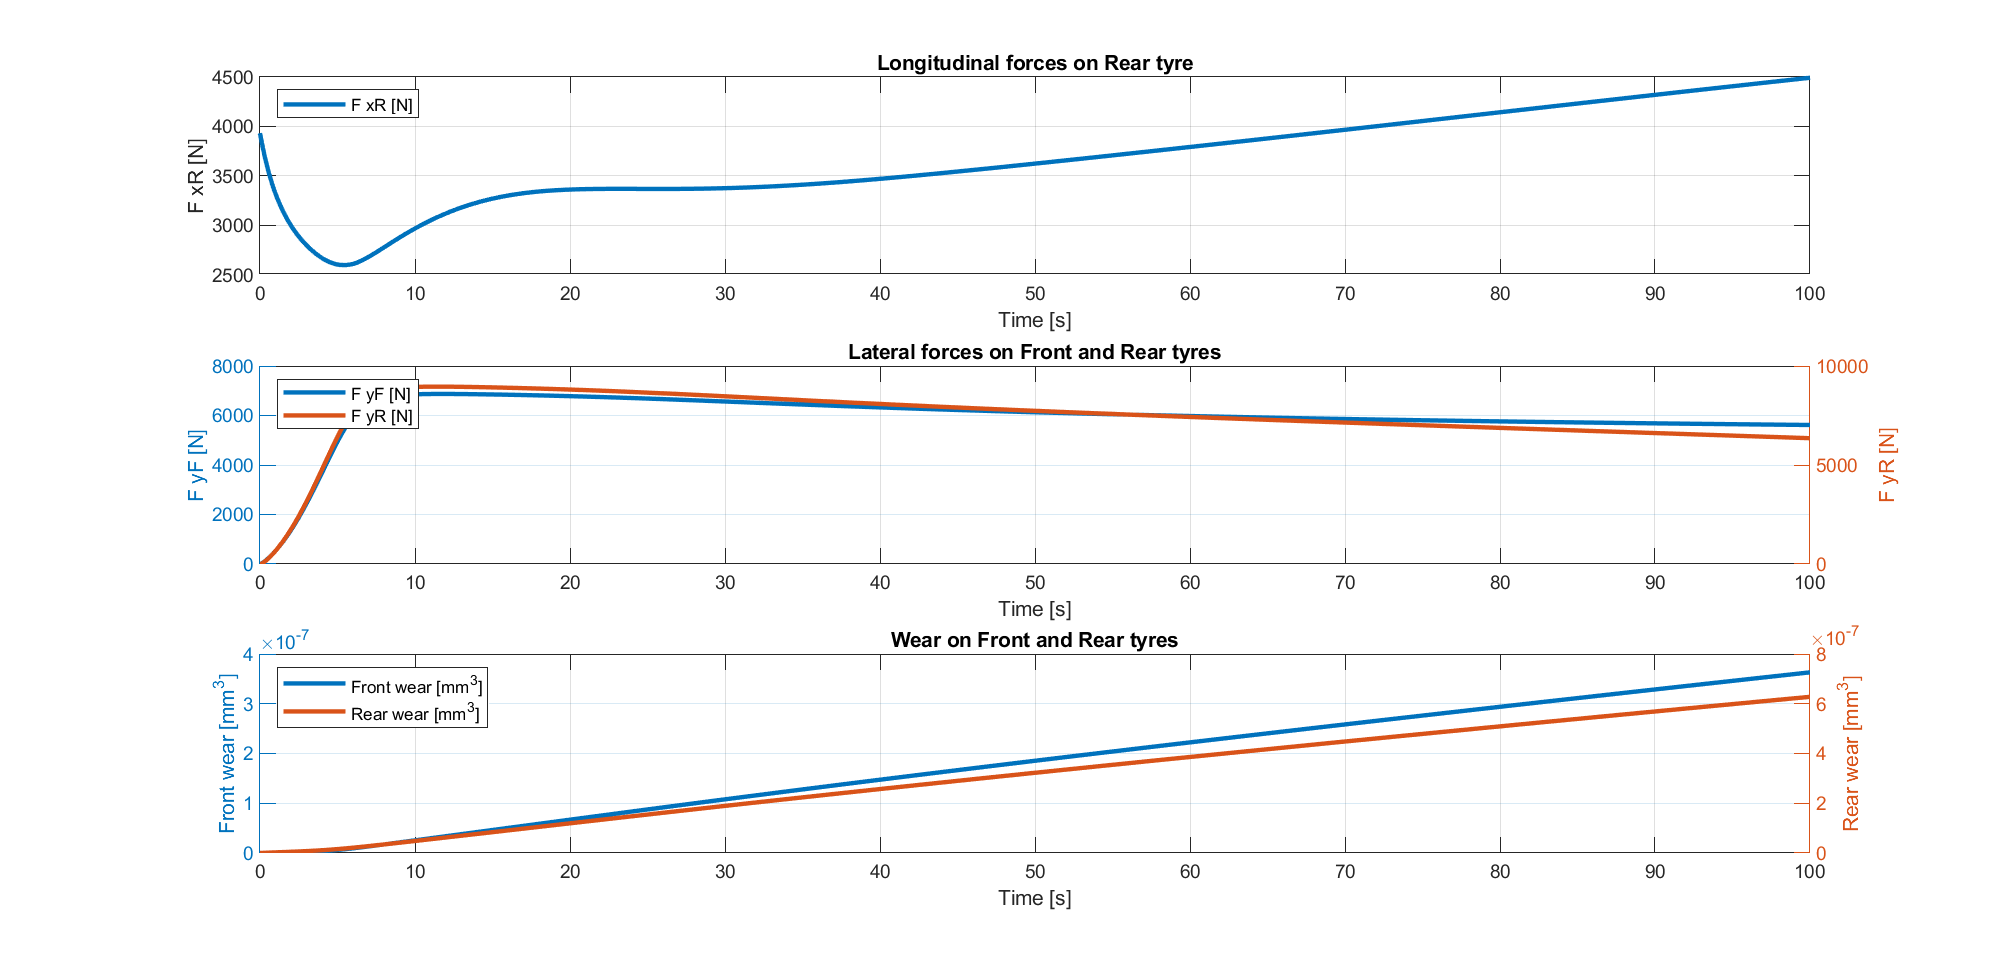
\includegraphics[width=\linewidth]{sim7_force-wear.png}
    \caption{Simulation 7 - forces and tyres wear figure}
    \label{fig:sim6_2}
\end{figure}
\begin{figure}[h!]
    \centering
    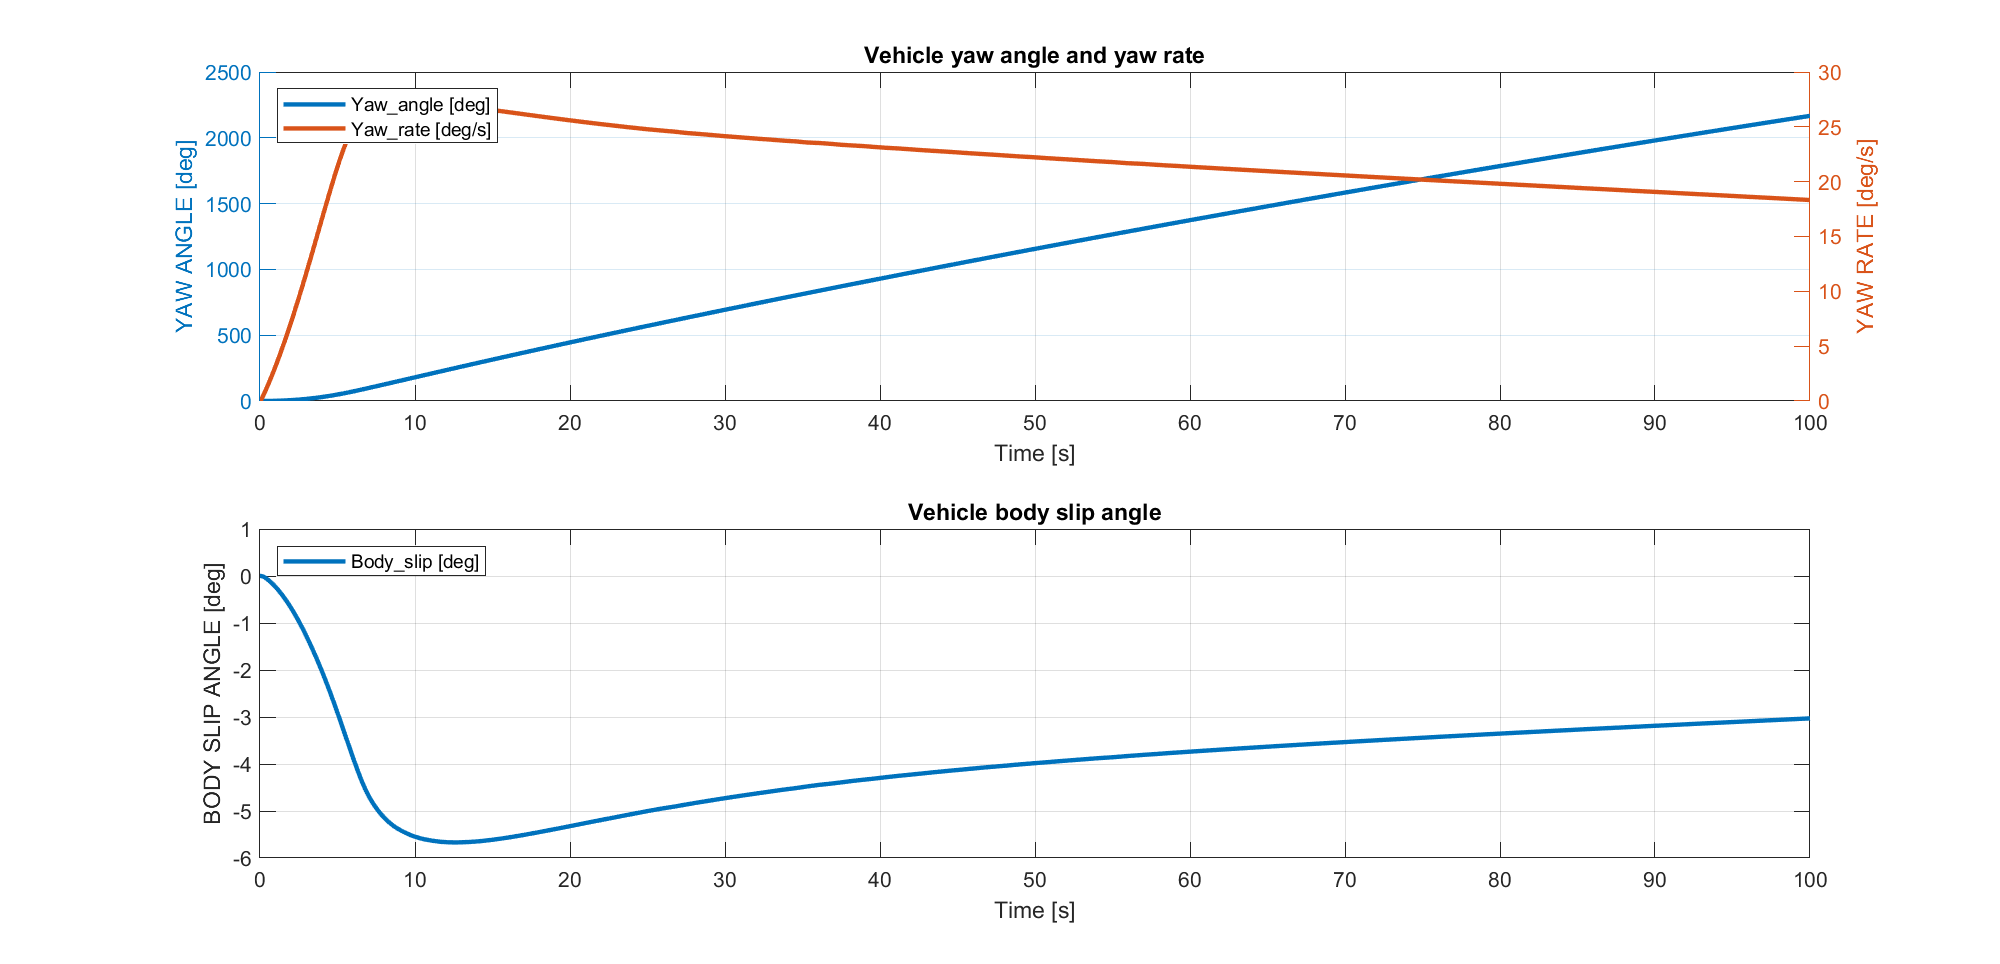
\includegraphics[width=\linewidth]{sim7_angles.png}
    \caption{Simulation 7 - angles figure}
    \label{fig:sim6_2}
\end{figure}
\begin{figure}[h!]
    \centering
    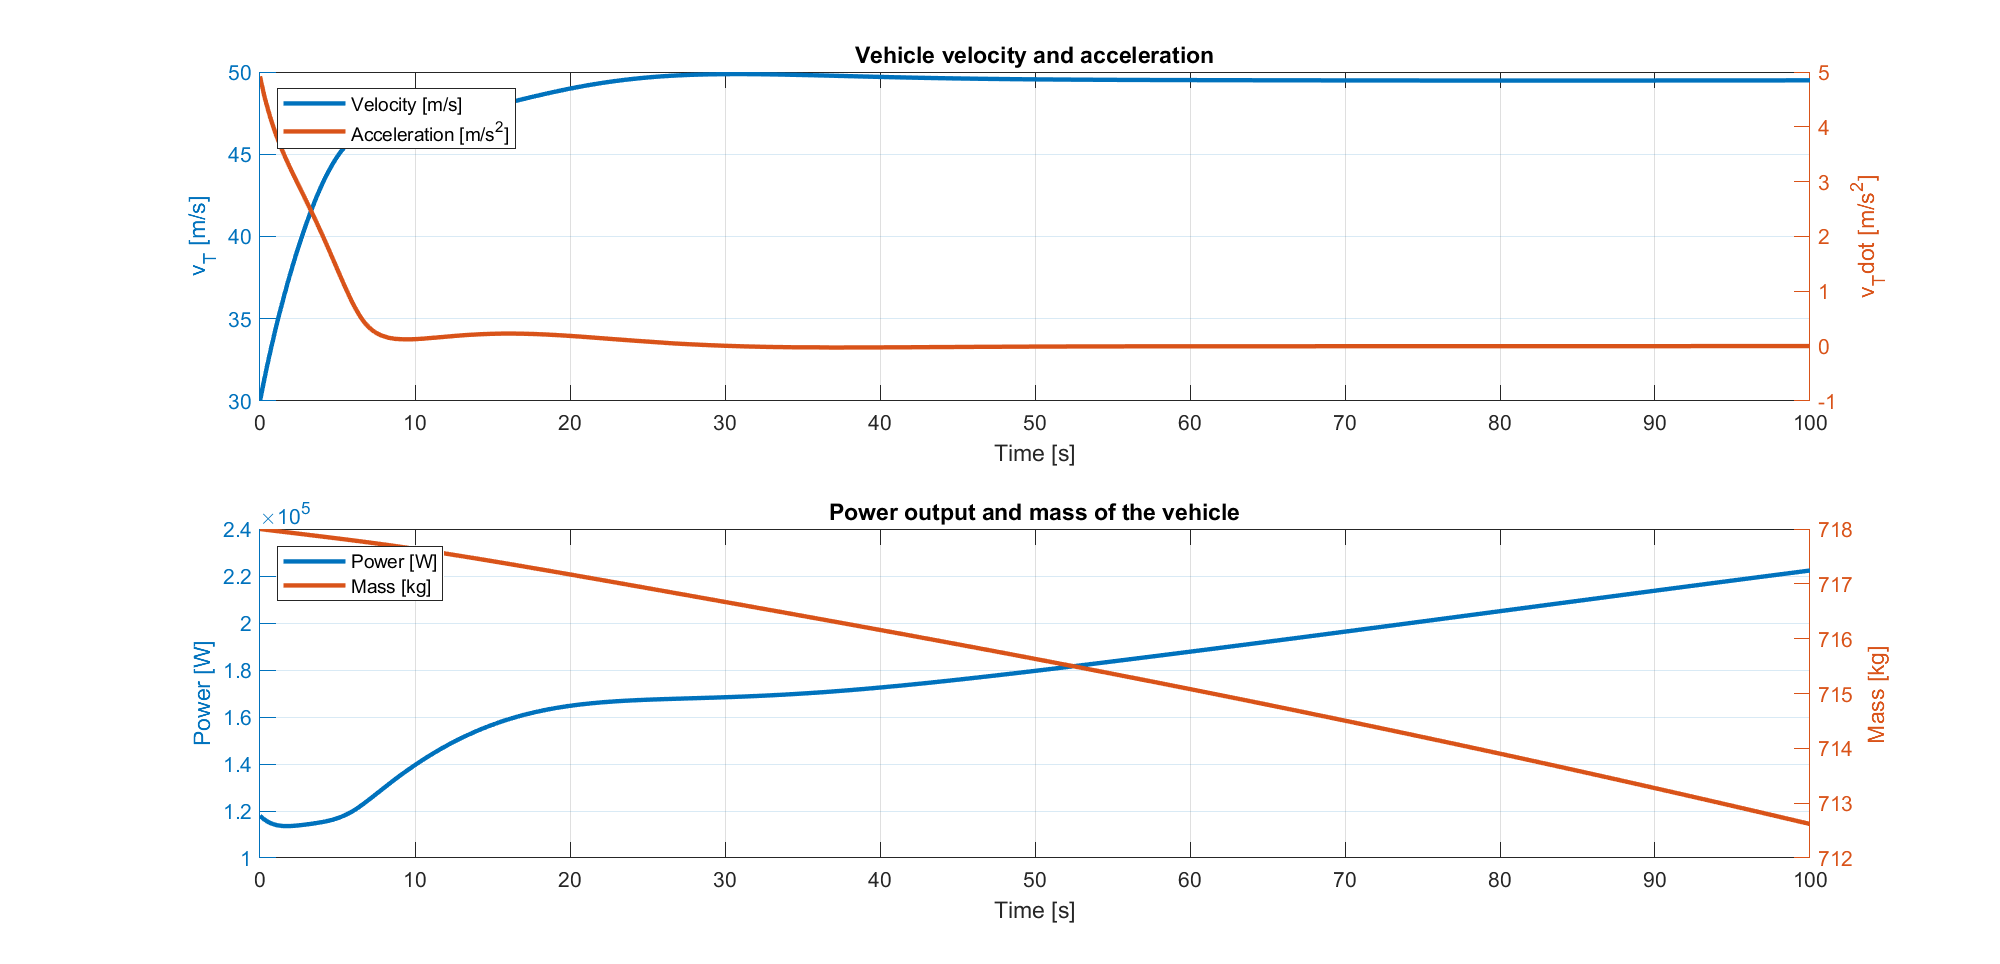
\includegraphics[width=\linewidth]{sim7_vel-power.png}
    \caption{Simulation 7 - velocity, acceleration, power and mass figure}
    \label{fig:sim6_3}
\end{figure}

\clearpage
\newpage

\section{Appendix}

In this section we will define the values given to the different parameters. 

\begin{equation*}
\begin{aligned}
\text{Parameters of lateral Pacejka tyre model}\\
a0 = 1.47 [-] \text{--------Shape factor}\\
a1 = 0 [1/kN] \text{--------Load influence on lateral friction coefficient (*1000)}\\
a2 = 2050 [-] \text{--------Lateral friction coefficient (*1000)}\\
a3 = 2500 [N/deg] \text{--------Change of stiffness with slip}\\
a4 = 10 [kN] \text{--------Change of progressivity of stiffness / load}\\
a5 = 0 [\%/deg/100] \text{--------Camber influence on stiffness}\\
a6 = 0 [-] \text{--------Curvature change with load}\\
a7 = -2 [-] \text{--------Curvature factor}\\
a8 = 0 [deg/kN] \text{--------Load influence on horizontal shift}\\
a9 = 0 [deg] \text{--------Horizontal shift at load = 0 and camber = 0}\\
a10 = 0 [-] \text{--------Camber influence on horizontal shift}\\
a11 = 0 [N] \text{--------Vertical shift}\\
a12 = 0 [N] \text{--------Vertical shift at load = 0}\\
a13 = 0 [N/deg/kN] \text{--------Camber influence on vertical shift, load dependent}\\
a14 = 0 [N/deg] \text{--------Camber influence on vertical shift}\\
a15 = 0 [1/deg] \text{--------Camber influence on lateral friction coefficient}\\
a16 = 0 [-] \text{--------Curvature change with camber}\\
a17 = 0 [-] \text{-------- 	Curvature shift}\\\\
\gamma = 0 [rad] \text{--------Camber angle}\\\\
\text{Parameters of longitudinal tyre model - only the ones used}\\
b1 = 0 [1/kN] \text{--------Load influence on longitudinal friction coefficient (*1000)}\\
b2 = 2080 [-] \text{--------Longitudinal friction coefficient (*1000)}\\
b11 = 0 [N] \text{--------Vertical shift}\\
b12 = 0 [N] \text{--------Vertical shift at load = 0}\\
\end{aligned}
\end{equation*}

\begin{equation*}
\begin{aligned}
m_{vehicle} = 590 [kg] \text{--------Mass of the vehicle}\\
m_{fuel} = 58 [kg] \text{--------Mass of the fuel}\\
m_{passenger} = 70 [kg] \text{--------Mass of the passenger}\\
m_T = m_{vehicle} + m_{fuel}+ m_{passenger} \\
g = 9.81 [\frac{m}{s^2}] \text{--------Gravity acceleration}\\
l_F = 0.414 [-] \text{--------Distribution of load on the front wheel}\\
l_R = 0.586 [-] \text{---------Distribution of load on the rear wheel}\\
a = 1.767 [m] \text{--------Distance between center of vehicle and front wheel}\\
b = 1.353 [m] \text{--------Distance between center of vehicle and rear wheel}\\
L = a + b [m] \text{--------Wheelbase}\\
I_T = 606 [kg m^2] \text{--------Moment of Inertia of the vehicle}\\
steering\_ratio = 10 \text{--------Steering ratio of the vehicle/tyres}\\
d_F = 0.8193*2 [m] \text{--------Front track width}\\\\
\end{aligned}
\end{equation*}

\begin{equation*}
\begin{aligned}
C_x = 0.725 [-] \text{--------Drag coefficient}\\
C_z = 0.778 [-] \text{--------Lift coefficient}\\
rho_{noslipstream} = 1.225 [\frac{kg}{m^3}] \text{--------Density of air without slipstream effect}\\
rho_{slipstream} = 0.8 [\frac{kg}{m^3}] \text{--------Density of air with slipstream effect}\\
S = 1 [m^2] \text{--------Area on which the air goes through}\\
distance\_threshold = 10 [m] \text{--------Front to rear distance for slipstream}\\
overlap\_threshold = d_F/2 [m] \text{--------Lateral overlapping threshold for slipstream}\\\\
\end{aligned}
\end{equation*}

\begin{equation*}
\begin{aligned}
%vel_{max} = 50 [\frac{m}{s}] \text{--------Maximum velocity of the vehicle}\\
%init\_vel = 20 [\frac{m}{s}] \text{--------Initial velocity of the vehicle}\\
%init\_xpos = 0 [m] \text{--------Initial y position of the vehicle}\\
%init\_ypos = -5.625 [m] \text{--------Initial y position of the vehicle}\\
%init\_yaw = 0 [rad] \text{--------Initial yaw angle of the vehicle}\\\\
C_{fuel} = 3x10^{-7} [\frac{s^2}{m^2}] \text{--------Fuel consumption coefficient}\\\\
K_{wear} = 1.3*10^{-17} [\frac{m^3s^3}{kg^2}] \text{--------Tyre wear parameter}\\
Tyre Contact Area Front = 0.072137 [m^2] \text{--------Contact area between front tyre and asphalt}\\
Tyre Contact Area Rear = 0.082758 [m^2] \text{--------Contact area between rear tyre and asphalt}\\
\end{aligned}
\end{equation*}

\begin{equation*}
\begin{aligned}
w_1 = 10^{-4.7} [-] \text{--------Parameter to scale ellipse due to wear}\\
w_2 = 1 [-] \text{--------Parameter to scale ellipse due to wear}
\end{aligned}
\end{equation*}

\chapter{Control}
\section{Longitudinal control}
\section{Lateral control}

\end{document}
